%% Modified documentstyle to documentclass -- compatibility with LaTex2e
%% N. Mancell (98/03/01).

%%  ucalgthes_root.tex        (NM 98/03/01)
%   Modified   92-09-18      Add references to dissertation        D. Teale
%                            Add approval page to toc
%                            Add ref to Title Degree on approval page
%   Modified  2006-09-12     Added geometry package to set up UofC thesis margins
%                            Removed includeprompt option N. Mancell               
%
\documentclass{ucalgthes1}   
\usepackage[letterpaper,top=1in, bottom=1.22in, left=1.40in, right=0.850in]{geometry}
\usepackage{fancyhdr}
\usepackage{multirow}
\fancyhead{}
\fancyfoot{}
\renewcommand{\headrulewidth}{0pt}
\fancyhead[RO,LE]{\thepage}  
%Define other usepackages here
\usepackage[plainpages=false]{hyperref}
\usepackage[pdftex]{graphicx}
\usepackage{fixltx2e}
\usepackage{amsmath}
\usepackage{float}
\usepackage{afterpage}

\title{Auto-tagging Emails and Instant Messages with User Stories to Build a Knowledge Base\\ 
\bigskip for Distributed Agile Projects}
%
%            Insert the correct information between the {}
%
\author{S. M. Sohan}
\thesisyear{2010}
\thesis{thesis}    % the word dissertation can be inserted between {}
\newcommand{\thesistitle}{Auto-tagging Emails and Instant Messages with User Stories to Build a Knowledge Base for Distributed Agile Projects}
\monthname{December}
\dept{COMPUTER SCIENCE}
\degree{MASTER OF SCIENCE}
%
%                    End of supplied information
%
\begin{document}
\makethesistitle
\pagenumbering{roman}     % resets page counter to one
\setcounter{page}{1}
\chapter*{UNIVERSITY OF CALGARY \\ FACULTY OF GRADUATE STUDIES}
\thispagestyle{empty}
The undersigned certify that they have read, and recommend
to the Faculty of Graduate Studies for acceptance, a \Thesis\ entitled
``\thesistitle'' submitted by \Author\
in partial fulfillment of the requirements for the degree of
\Degree.\\

%
%                 Substitute  List of Examiners
%
\begin{signing}{Department of Academic Computing}
\signline
Supervisor, Dr. Frank Oliver Maurer \\
Department of Computer Science \\
\signline
Dr. Jonathan P. Sillito\\
Department of Computer Science \\
\signline
Dr. Xin Wang \\
Department of Geomatics Engineering \\
\end{signing}
%
\newpage
\phantomsection
\altchapter{Abstract} 
In distributed agile teams, people often use email and instant message as knowledge sharing mediums to clarify the project requirements or user stories. Knowledge about the project included in these private mediums is easily lost when recipients leave the project. This thesis presents a new machine learning based technique, Taggy, to retain knowledge from emails and instant messages. Taggy automatically captures project related emails and instant messages and tags with the relevant user stories based on their context and text relevance. This auto-tagged knowledge may be useful for different purposes such as training new team members, re-engineering an application and so on. This thesis presents the auto-tagging technique, Taggy, with its prototype implementation and evaluation results based on 4,757 emails from 9 agile teams and a preliminary user study of 6 participants. The challenges and limitations are also discussed, some of which are enlisted as potential future work on this topic.
\newpage

\phantomsection
\altchapter{Acknowledgements}
I have been blessed with the trust and support of a number of people and organizations while working on this research. In this regard, I would like to thank -

Dr. Frank Maurer and Dr. Michael Richter for your help with formulating and advancing this research. You have provided me with useful guidelines and suggestions at various steps and kept trust in me all the way.

Syed Rayhan and the Code71 team for providing me with an excellent environment for learning and innovative thinking. Working with you have been a memorable experience and helped me coming up with this research idea.

University of Calgary for your financial support without which I couldn't carry out this research.

My loving wife, Shahana, for giving me a happy family life. You have come all the way from Dhaka to Calgary to accompany me and that proved to be a lot for my well being.

My parents, S. M. Afaz Uddin and Mrs. Kh. Shirin, for inspiring me all through my life. Your continuous inspiration has given me the enthusiasm and courage at all walks of the life and this graduate research is one example of that.

Bangladesh, my country, for your promise to educate and raise me. You have given me the strong foundation to face the world.

\newpage

\phantomsection
\altchapter{Publication} 
The core ideas of this thesis appeared in the following publication:

\begin{quote}
	S. M. Sohan, Michael M. Richter, and Frank Maurer. Auto-tagging emails with user stories using project context. In Agile Processes in Software 	Engineering and Extreme Programming, volume 48 of Lecture Notes in Business Information Processing, pages 103 - 116. Springer Berlin Heidelberg, 2010.
\end{quote}



\begin{singlespace}
\newpage
\phantomsection
\tableofcontents
\pagestyle{plain}
\newpage
\phantomsection
\listoftables
\pagestyle{plain}
\newpage
\phantomsection
\listoffigures
\newpage
\altchapter{Epigraph}
\begin{quote}
If I'd had some set idea of a finish line, don't you think I would have crossed it years ago? 	
\end{quote}

Bill Gates

\pagestyle{plain}
\clearpage
\end{singlespace}
\clearpage          % otherwise tables will be numbered wrong

\pagenumbering{arabic}


%!TEX root = /Users/smsohan/Taggy/Thesis/ucalgthes1_root_0.tex
\fancyhead[RO,LE]{\thepage}
\fancyfoot{} 
\chapter{INTRODUCTION}
Agile software engineering process is a collaborative approach to incrementally deliver software in small iterations (e.g. two to four weeks). Agile teams commonly use ``user stories'', a small description of a desired feature in everyday language, to capture the requirements. An example user story is as follows:\\
\begin{quote}
\emph{As a shopper, I want to pay online to checkout my shopping cart using MasterCard, Visa or Amex credit card from a secured web page only.}\\
\end{quote}
The details of such user stories are discussed as an ongoing basis among the people involved in a project. For example, as the engineering team start working on the stories, they often consult with customers and other teammates to further clarify such user stories. Whenever possible, face-to-face communication is preferred as the principal communication medium between customers and developers in agile processes \cite{am} \cite{xp} \cite{scrum} \cite{xp_up}. In collocated setups, where the people work in close proximity, such informal communication relays the tacit knowledge among the people. 

However, for distributed projects, especially when there is a huge time zone difference among people, face-to-face communication become infeasible. As a result, people use alternatives to mitigate this shortcoming such as phone calls, emails, instant messaging, wiki, web forums and so on. So, in such setups communication is often text based instead of tacit knowledge sharing. In this sense, distribution makes it easy to capture the knowledge since much of it is textual and electronic. For an example, considering the aforementioned user story, the developer may send the following email to the customer to further clarify expectations.\\

\begin{quote}
\emph{\textbf{Subject:} Clarification required on online credit card payment\\
\textbf{Hi Bob:}\\
Please clarify if the shoppers need to provide the security code of the credit card while doing checkout.}
\end{quote}

Since email is a persistent tool, one can use this knowledge in future. But, email is also a personal tool and its hard to transfer a selection of project related emails from the rest in a reusable format. The same is true for instant messages as well. So, when someone leaves the team, it becomes hard to access that knowledge when needed later down the road. To retain these useful knowledge, this thesis implemented and evaluated a tool called \textbf{``Taggy''} that automatically grabs and tags the emails and instant messages with relevant user stories.

The relationship between a user story and email or instant message is not explicit. To establish the implicit relation, Taggy uses a machine learning technique, Case Based Reasoning (CBR). The CBR system looks at the text, people and temporal similarity between emails and user stories. The evaluation results show that a well trained software can auto-tag emails with user stories. Also, we found that combining context information with text similarity helps to find the related user stories with higher accuracy than using just text match alone.

In the existing literature attempts have been made to capture software project related knowledge following several alternative approaches. For example, commercial tools exist that link software code commit messages with a requirement or ticket given the ticket number is present inside the commit log. Also, another approach is to use wiki or online message threads, where the contents are manually linked with the user stories. However, to use such approaches, one needs to remember identifiable tokens or learn markup syntax (e.g. wiki), which is often burdensome for business users. To reduce this learning curve and human efforts, Taggy builds a knowledge base by automatically tagging emails and instant messages with user stories. 

The remaining part of this chapter is organized as follows: First, I discuss the necessary background material about user story and distributed agile projects to develop a shared understanding of the terms used in this thesis. Then, the research motivation is discussed. Finally, I present the research goals and related challenges.

%Start the body text
\section{User Stories - An Overview}
In agile projects, user stories are used to capture requirements. In short, user stories represent the need for a feature from the view point of a potential user of a software. Mike Cohn \cite{user_stories_applied} defines user stories as follows:\\
A user story describes functionality that will be valuable to either a user or purchaser of a system or software. User stories are composed of three aspects:
\begin{itemize}
	\item a written description of the story used for planning and as a reminder
	\item conversations about the story that serve to flesh out the details of the story
	\item tests that convey and document details that can be used to determine when a story is complete
\end{itemize}

As outlined in the above definition, conversation plays a central role in fleshing out the details of the user stories. Ron Jeffries \cite{ron_jeffries} and Rachel Davies\cite{rachel_davies} also emphasize the role of conversation being a key component of user stories.

Wake, author of \cite{bill_wake}, suggested another popular acronym, INVEST, that defines good stories being Independent, Negotiable, Valuable to users, Estimable, Small and Testable. However, to hold all these characteristics yet being Small essentially points to conversation as means of detailing the user stories.

In an agile project, the customer or a representative of the customer is responsible for coming up with these user stories with the help of the stakeholders. Next, the user stories are prioritized in a list known as ``Product Backlog''. At every iteration (typically two to four weeks), the team picks the top user stories from the product backlog known as ``Iteration Backlog'' with the target to deliver the user stories at the end of the iteration. A user story is supposed to be limited to a scope so that it can be delivered within the iteration. However, the details about the user stories are laid out as on going basis during the iteration through customer collaboration and feedback.

One or more team members are assigned to deliver a user story, which may involve design, development, testing and such tasks. It is a common practice that the customer and the assigned people collaborate to fine tune the user story details. Collocated teams often use sticky pads on a team wall or whiteboard to stick the iteration backlog and visualize progress. Figure~\ref{fig:scrum_wall} shows a Scrum Wall, where user stories are grouped based on the development status:

\begin{figure*}[bt]
	\centering
	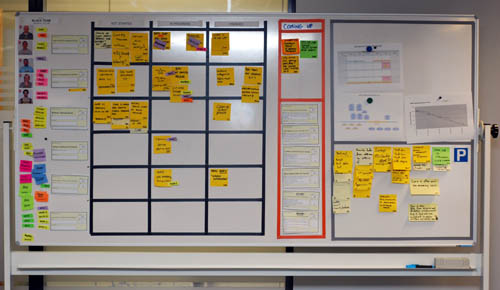
\includegraphics[width=\textwidth]{ScrumWall.jpg}
    \caption{A Scrum Wall. Source: http://www.xqa.com.ar}
	\label{fig:scrum_wall}
\end{figure*}

However, distributed agile teams often use virtual team walls in place of the physical wall so that it is usable across several geographical locations. Figure~\ref{fig:target_process_wall} shows such a virtual wall taken from ScrumPad:

\begin{figure*}[bt]
	\centering
	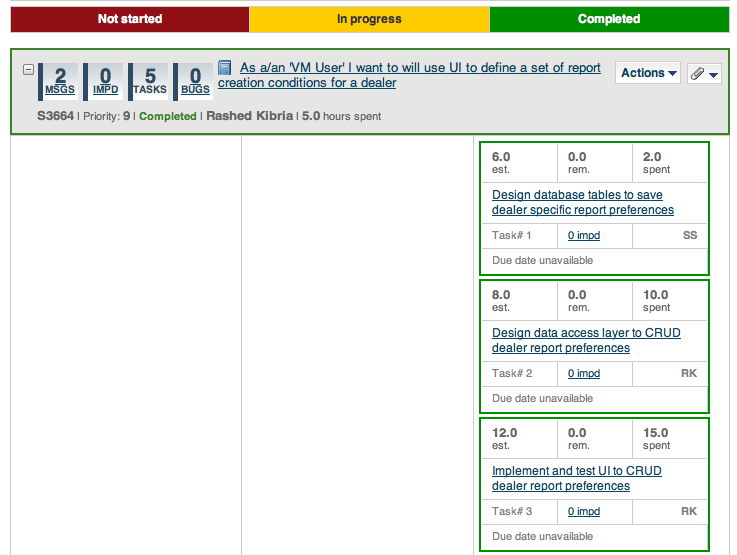
\includegraphics[width=\textwidth]{ScrumPadWall.png}
    \caption{A Virtual Scrum Wall. Source: http://www.scrumpad.com}
	\label{fig:target_process_wall}
\end{figure*}


\section{Distributed Agile Projects}
The members of a distributed agile project work from different geographical locations and adopt agile principles. In practice, the distribution can take several models such as the following three outlined by Braithwaite et al \cite{xp_expanded}:

\begin{enumerate}
	\item Agile outsourcing - the development team is offshore to the customer.
	\item Agile dispersed development - developers spread over different locations, such as open source projects.
	\item Distributed agile development - customers are distributed and one development team is distributed evenly to stay close to the customers.
\end{enumerate}

Again, the geographical distribution can be anywhere between offices across the road to opposite part of the world. For example, a team may work for a customer at the same city or a country separated by ten hours of time zone difference. Distributed agile teams often use different electronic communication channels such as Emails, Instant Messaging, Wiki and Forums as well as online project management tools to uncover the important details about the user stories.

\begin{figure*}[bt]
	\centering
	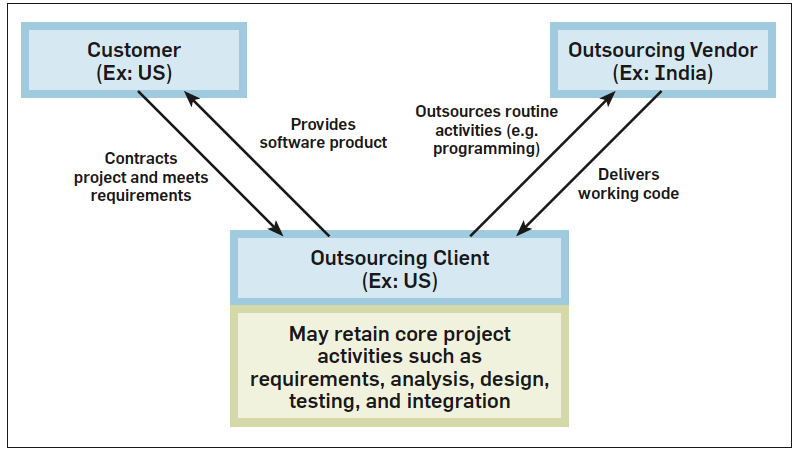
\includegraphics[width=\textwidth]{Distributed.png}
    \caption{An Example Agile Outsourcing Model. Source: \cite{modified_agile}}
	\label{fig:distributed}
\end{figure*}

Figure~\ref{fig:distributed} shows an example of an outsourced agile project taken from \cite{modified_agile}. Similar to this one, a distributed agile project may employ people working on different roles across the globe.

Cost savings has been identified as one of the principal deciding factors for distributing projects across the globe \cite{practical_considerations}. However, projects also go distributed to utilize global talent supply and local knowledge \cite{fully_distributed, modified_agile}. Previous studies have reported success with distributed agile projects. For example, Sutherland et al. reported a linear scalability with a globally distributed outsourced team following a Fully Distributed Scrum (Scrum is a popular agile method) model \cite{fully_distributed}. Similarly, Yahoo! had success with distributed teams that valued people over process and exercised the right information sharing formats and timing \cite{yahoo}.

To ensure a shared view of the ``Product Backlog'' and ``Iteration Backlog'' distributed teams often use web based project management tools. There are a number of such tools available commercially as well as open-source \cite{scrum_pad, version_one, xplanner, trac}. Such tools help people working remotely to have a single backlog and collaborate around that. 

\section{Research Motivation}
The existing literature about collaboration in distributed agile software projects suggest the use of various electronic mediums to counter for missing face-to-face communication. Because of time zone difference, such teams often use asynchronous communication tools such as email and wiki in addition to synchronous ones such as telephone call, instant messaging etc. For example, Robarts \cite{practical_considerations} found that teams would follow up with a written email after they had a telephone meeting to ensure the message is clearly understood. Moreover, of all the available written communication tools, email has been regarded as the most-widely used one by several former studies \cite{collaboration_in} \cite{on_coord}. Additionally, even in collocated settings, people often use emails to communicate as it doesn't require immediate response and overheads like scheduling meetings.

Although having multiple communication channels adds flexibility for collaboration, it also means the knowledge gets fragmented across different channels. This fragmented knowledge may be spread over the project management tool, wiki, emails, instant messages and other places. Basili et al. provided the following list of experiences related to the lack of access to available information \cite{implementing_an_experience}:

\begin{itemize}
	\item An employee left with short notice. The organization lost all of its experience in a certain area and tries to recover it, but it doesn't even know what experience was lost.
	
	\item A consultant spends three weeks developing a course that already exists because he doesn't know that it was done before.
	\item Someone repeats a \$35,000 mistake for which there is a simple solution.
	\item A consultant gave a customer a promise, but is now busy with other work. No one else knows about his promise so it doesn't happen.
	\item An employee learned a lot during a project, but has no time for packaging and dissemination so the knowledge cannot be leveraged.
	\item A new employee is hired, but is for a long time considered a burden instead of help because he needs detailed support from his coworkers, who do not have sufficient time to help him.
	\item (continued...)
\end{itemize}

For agile teams, this situation can be improved with a useful knowledge management solution. To retain the important details about the user stories, one needs to combine these fragmented pieces. But looking into email inboxes of colleagues may be obtrusive to their privacy, if not impossible. Even worse, when a teammate leaves, the emails are gone as well. So, the fragmented pieces of knowledge is either lost or very hard to combine together. Even if one has access to the emails, manually copy-pasting all the emails and combining with the relevant user stories would be a time consuming task to say the least. The following user story and email collaboration shows an example of the knowledge fragmentation:

\begin{quote}
	\textbf{Available in Project Management Tool}\\
	\textbf{User Story}\\
	\textbf{Title:} ``As a/an VM System I want to load Auction data from NADA data file''\\
	\textbf{Description:} Please see the 3 documents related to Auction data
	\begin{enumerate}
		\item Auc Layout
		\item \textbf{Regions Table}
		\item AucData.zip
	\end{enumerate}
\end{quote}

In this example, the user story represents a data integration with a company named NADA. NADA provides vehicle auction information for regions denoted by a ``region code''. However, as the developer starts working on NADA integration, she asks the following question about the region code to the customer through email. 

\begin{quote}
\textbf{Email\#1 (From Developer to Customer)}\\
\textbf{Subject:} ``Initial Questions regarding NADA region value''\\
\textbf{Body:} We found that the Region value can be \textbf{Alpha-numeric} that will be received from NADA Auction. But, the NADA WS accepts only \textbf{Numeric} Region value. Is there any conversion rule to convert the region value into numeric? \\
Thanks
\end{quote}

To answer this question, the customer replies with the following email.

\begin{quote}
\textbf{Email\#2 (From Customer to Developer)}\\
\textbf{Subject:} ``RE: Initial Questions regarding NADA region value''\\
\textbf{Body:} I talked to NADA and they provided me with the \textbf{attached conversion table} for \textbf{Alpha-numeric} to \textbf{Numeric} region codes.
\end{quote}

Please note that the email from the customer included a conversion table for ``region codes''. 

Given this example, if a person only looks at the user story, she will find partial information about it. So, the whole conversion of ``region code''  may be confusing to her. However, when she can see the emails along with the user story, she may have a better understanding about this user story.

This information may be required since a distributed agile team have to cope up with changes in team composition as new people will join and some people may leave. So, if it is possible to combine the fragmented knowledge from different places such as emails, instant messages and project management tools, one can find the important details of the user stories. Such details may not be obvious when only the user story is available. Similarly, the knowledge can help in testing of the features since it is expected to contain customer feedbacks and clarifications on user stories.

The motivation for this thesis stems from the pursuit of developing an agile knowledge base by combining the fragmented knowledge from emails, instant messages and project management tools with the least possible human efforts.

\section{Research Problem}
In software development projects, developers sometimes leave the team for various reasons. As said before, in distributed agile projects, important knowledge is often shared by emails. To transfer this knowledge for future use, one first needs to find the project related emails. Secondly, in such setups people often use web based project management tools to capture user stories and planning information. If the emails can be related to specific user stories in the project management tools, then another developer of the team will be able to easily find the necessary information about a user story when required.

From an end users' point of view, manually finding and relating the emails with user stories is a time-consuming and costly process. This essentially means copying the emails from inbox and putting into a system and linking with a user story. This manual process is cumbersome to say the least. However, if a software can do this, then it may work as a knowledge-base even after someone leaves the team. Such a software needs to be unobtrusive for the most part so that it doesn't require much human effort. So, a technical solution needs to be in place that can capture the project related communication without violating people's privacy. For example, it cannot look into the email inbox of a developer nor should ask a developer to manually enter the chat log into the system.  

The core technical challenge in devising such a software solution is understanding the emails and relating them to specific user stories. The relation between an email and a user story is not explicit. Alternative approaches to make it explicit, such as using identifiable tokens in email subjects, also makes the communication process obtrusive as it adds an extra step to lookup the identity or memorizing it before writing an email. To alleviate this extra step, one can modify email clients to do the lookup. But doing so for the multitude of emails clients including the ones on mobile phones is cumbersome. Also, it imposes a behavioral change or a learning curve for the for the people at the business end.

To find out the implicit relation between a free-format email and a use story, a software needs to handle similarity between two texts, which is a standard problem. Emails may not show very high text similarity with the related user stories. This text component makes the relevance between a user story and an email an approximation or fuzzy match. Also, pure text retrieval limits how accurate the assignment of email and user stories can be. This is because people use different vocabulary and often a tacit communication is there underneath a written form. Using context information has the potential to increase this accuracy. So, a software needs to be able to combine both the text and context similarity for auto-tagging emails with user stories.

To account for the context, one needs to use the associated meta information that are available. The contexts of an email and a user story are not exactly similar. For example, the context of an email has a time-stamp, sender, recipients and past conversations. On the other hand, user stories have a different context, such as their development time or iteration timeframe, developers and customers. An auto-tagging solution needs to use these context meaningfully so that each component gets its deserving share of importance in the relevance computation. So, it is important to have a formula that produces similarity ranking considering the fuzzy text similarity and associated context relevance.

Next technical challenge is to evaluate the accuracy of the auto-tagging system. For the auto-tagging to be useful, it shouldn't make too many mistakes in finding similarity. The accuracy of this system needs to be tested using real world data. 

Another technical challenge is to design an adaptive auto-tagging system so that it can adapt to different communication patterns. Since distributed agile teams across the world have differences in who, how and when they communicate about their user stories, the auto-tagging system needs to adjust its similarity computation accordingly. For example, one team might spend more time communicating about user stories that are currently under development while another team might prefer to discuss about the upcoming ones. An auto-tagging system that uses the meta information of time needs to learn this pattern to make a right decision.


\section{Research Goals}
\begin{figure*}[bt]
	\centering
	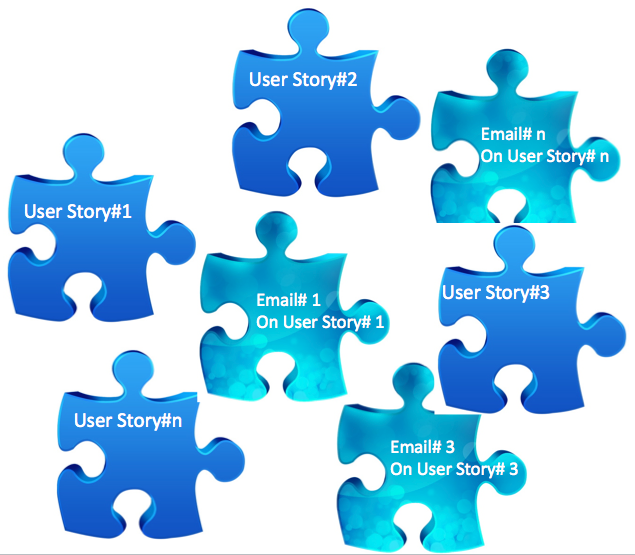
\includegraphics[width=\textwidth]{Jigsaw.png}
    \caption{Jigsaw Puzzle Visualizing the Auto-Tagging Problem}
	\label{fig:jigsaw}
\end{figure*}

The principal goal of this research is to develop a tool that can automatically read and relate emails with user stories based on agile project context. The tool needs to minimize human efforts in doing so. Another complementary goal is to evaluate the tool using real world data. The underlying approach and evaluation of Taggy is discussed in Chapters ~\ref{ch:taggy} and ~\ref{ch:evaluation}.

Figure~\ref{fig:jigsaw} visualizes the research goal as it shows the fragmented knowledge from project management tools and email inboxes to be combined in a jigsaw puzzle. The target is to solve this puzzle so that each user story gets connected to the relevant project related emails.

This research also aimed to investigate the difficulties in solving the various aspects of the research problem, namely i) relevance ranking of user stories for a given email, ii) using text similarity in addition to context relevance, iii) evaluating auto-tagging accuracy and iv) developing an adaptive auto-tagger. The findings from this investigation is expected to provide a foundation for next level of research in this area.

\section{Key Contributions}
This research work has been published and presented at XP 2010 \cite{auto_tagging}. 

The key contribution of this research is, it demonstrates a novel approach of building a knowledge-base for distributed agile teams from emails and user stories. This approach has the similar motivation as found in some previous works, such as clustering emails archives\cite{using_hybrid}, tagging forum messages with source code change set\cite{hipikat, hipikat_2} and using wiki to share knowledge. However, this research shows a machine learning approach to conglomerate fragmented knowledge from emails, instant messages and project management tools minimizing human efforts. This new technique adds to the existing body of knowledge.
                                  
Another key contribution is, it shows that text and context similarity can be used to find relevance between two different types of entities such as emails and user stories, where the degree of text similarity may be inadequate. We have used Case Based Reasoning (CBR) for auto-tagging. As this research findings suggest, other CBR systems concerning different entities may utilize this technique.

%!TEX root = /Users/smsohan/Taggy/Thesis/ucalgthes1_root_0.tex
\fancyhead[RO,LE]{\thepage}
\fancyfoot{} 
\chapter{Related Work}
\label{ch:related_work}
Researchers have attempted to solve the problem of knowledge management for software development projects from different points of view. Also, the industry is using a number of available commercial and open-source tools to retain and manage knowledge. To find the similarity and contrast of this research with the existing approaches, this related work chapter is divided into sections dedicated to the following five areas:

\begin{enumerate}
	\item Communication in distributed teams
	\item Capturing knowledge from emails
	\item Wiki-based knowledge sharing
	\item Context-based knowledge management
	\item Review of existing tool support for knowledge sharing
\end{enumerate}

\section{Communication in Distributed Teams}
The Agile Manifesto \cite{am} puts heavy emphasis on customer collaboration. Understandably in distributed projects, geographic and temporal distances create communication challenges not seen in a collocated setup. Existing research focuses on the use and effectiveness of the different communication channels that are used in distributed projects.

Thissen et al. points out that for a distributed team to become successful, it must use appropriate tools to ensure easy flow of information \cite{communication_tools}. Lanubile provided a categorization of such collaboration tools \cite{communication_in_distributed} that include software configuration management, bug and change tracking, build and release management, product and process modeling, knowledge center and communication tools. Lanubile also pointed out that asynchronous communication tools include emails, mailing lists, newsgroups, web forums and blogs while synchronous ones include telephone and conference calls, chat and video conferencing. Of all the asynchronous tools, they identified email as the most widely-used and successful collaborative application because of its flexibility and ease of use.

The use of synchronous vs. asynchronous mediums depends on teams and their temporal as well as geographical distance. For example, Hole et al. found that teams often preferred email and instant message over telephone calls for meeting between two sub-teams at two different locations due to language barriers \cite{a_case_study_of}. Here is an excerpt from a Scrum Master, one of the participants of their study:\\

\begin{quote}
``we tried to use telephone conferences, but it did not work well, because of language problems. It is also easier to understand each other when relying on written communication. Also extensive use of chatting makes it possible to ask a question right away. It takes time to organize a telephone-conference.''
\end{quote}

Korkala et al. found that despite the availability of richer communication media, the customers preferred to use emails for most of their mid-iteration communication needs\cite{communication_in_distributed}. Here is an opinion from a customer of their case study about the selection of a medium for mid-iteration communication:\\
\begin{quote}
	``Emails will do just fine. They are enough.''
\end{quote}

Chau et al. suggested that a shared ownership of knowledge center fosters team participation \cite{knowledge_sharing}. This is because the responsibility is of creating and updating the knowledge is distributed and one does not need to go through the process of approval while contributing to a knowledge base. However, they identified that keeping the knowledge up-to-date is an important issue. To build a lightweight medium for retaining explicit knowledge and provide easy access, they suggested the use of wiki. They also pointed the fact that, in agile teams the key portion of knowledge sharing takes place through autonomous interaction. So, much of the explicit knowledge sharing is actually done via the channels that are frequently used for communication.

Hildenbrand et al. suggested that customers and testers of distributed agile teams need to work closely to flesh out acceptance criteria for user stories in the iteration backlog \cite{agile_methods}. Also, quick feedback from customers is needed during the design and development of a user story. They also emphasized that this knowledge could be of great use and must be shared with the whole team. To collaborate and capture this knowledge, they suggested the use of online groupware and instant messaging.

Cataldo et al. looked into the types of knowledge contained in the emails of a distributed project and found that email was the most preferred medium for information exchange and task negotiation related topics\cite{on_coord}. Although the target was to use groupware for such activities so that the knowledge could be easily retained and shared, their data suggests that developers relied heavily on emails for information acquisition. Layman et al. classified the emails exchanged in a distributed agile project into several types such as: i) changes in specification, ii) clarification, iii) prototype, iv) feedback, v) planning/scope, vi) bug, vii) acceptance test and viii) post-release bug related emails \cite{essential_communication}. They also found that clarification related emails were the most frequently exchanged of all these categories. Figure~\ref{fig:layman} shows their findings for twelve iterations of a project.

\begin{figure*}[h!]
	\centering
	\includegraphics[width=\textwidth]{Layman.png}
    \caption{Use of Emails for Different Purposes. Source: \cite{essential_communication}}
	\label{fig:layman}
\end{figure*}

To summarize, this section of the literature review suggests that distributed teams often use emails and other text-based asynchronous mediums alongside real-time collaboration tools to share important knowledge about their projects. Based on these findings, this thesis emphasizes on automatically capturing project related emails and instant messages and linking them with relevant user stories. Since emails and instant messages are widely-used to share knowledge among people in distributed projects, the solution shown in this thesis can be used to retain and reuse this knowledge.

\section{Capturing Knowledge from Emails}
In the existing literature, there have been attempts to extract knowledge by mining software project related emails. Largely, the concentration of such mining efforts has been around clustering the archives into meaningful groups. Also, there has been work around the visualization of email archives so that one can easily navigate the corpus of emails.

Berlin et al. designed and implemented a group memory system called TeamInfo \cite{where_did_you}. TeamInfo let people to use the CC: (or carbon copy) feature of emails to forward a project related email to the TeamInfo system. Once TeamInfo reads the email, it finds the predecessors, if any, and tries to classify the email into one of the preset categories. These preset categories are similar to what we see in email folders or filters, namely grouping by one or more of conditions involving sender, recipients, subject and text containment. This classification is intended to help in browsing the emails based on their high level categorization. However, the users of TeamInfo faced challenges to come up with the right categorizing conditions as at times one email could be part of multiple categories. Also, a fine grained categorization would lead to hundreds of such classes, which, again, makes it hard to easily browse to a topic of interest. To write a filter, TeamInfo requires significant experience as the rules are expressed using a new declarative language. TeamInfo helped its users in retaining and sharing knowledge. Taggy is similar to TeamInfo in that it uses the same CC: feature of emails to get hold of the knowledge. But the key difference is, instead of asking the users to provide rules for classifying emails, Taggy tries to tag emails with relevant user stories. Taggy is designed to help agile teams, where the presence of assigned developers, customers and time box provide a context to the plain text-based user stories. As a result, instead of trying to group the emails, Taggy tries to automatically link up emails with the user stories so that one can follow the discussions related to specific features of a software. This alleviates the overhead of creating and managing shared grouping rules as well.

A knowledge-base is often used to recommend a developer about required source code change locations. Hipikat is such a recommender that uses interlinked information from several sources, such as CVS log messages, online documents and newsgroup threads \cite{hipikat}. Here, the newsgroup threads are essentially the group emails exchanged among people working on a project. To infer the relationship between a thread discussion and other artifacts, Hipikat uses ``References'', a header element that can identify the thread's topics of interest. However, in agile projects such email threads are often exchanged between customer and developers and it might require extra effort either to memorize or to lookup the ``References'' identity every time before starting a discussion. Taggy emphasizes seamless customer collaboration and reduces this extra lookup cost through utilizing machine learning techniques to infer the hidden relation between an email and user story.

Existing research also looked into mining and visualizing the contents of software related email archives to extract important patterns. For example, Medynskiy provided a multi-modal visualization of email, instant message and CVS commit logs from the Python project\cite{using_hybrid}. They mined the textual information to extract meaningful groups and linked among the groups to content contributors. This way, one could navigate related knowledge from different sources that are otherwise fragmented. In effect, Taggy also tries to unite the fragmented pieces of information. But the concentration is at a higher level (user stories) as opposed to lower level artifacts (CVS logs). Also, instead of mining archived data sources, Taggy builds the knowledge-base as it is created.

Another work, The Experience Factory implementation introduces several tools for capturing emails and instant messages \cite{implementing_an_experience}. For example, they capture Frequently Asked Questions with expert answers, focused chat sessions, email and project related presentations. However, the management activity in Experience Factory requires human efforts to collect the email contents into the system as well as keep them updated. Taggy addresses this issue by not only automatically grabbing the emails but also using a machine learning approach to tag emails with user stories.

Software requirements traceability helps developers to understand a requirement based on its underlying reasoning \cite{automating_requirements}. However, for distributed agile projects, this is hard since knowledge is dispersed. Tagging emails with user stories could improve the traceability in such cases. To attain this goal, the approach of Taggy is in alignment with the aforementioned research into building a knowledge-base from emails. However, it is extended to be used in agile projects, where the use of available context helps the computer to make an informed guess about if an email is related to a user story or not.

\section{Wiki-Based Knowledge Sharing}
The overwhelming success of Wikipedia \cite{wikipedia} is a result of collaborative editing. Being inspired by this, several researchers explored the potential of using Wiki for collaborative software knowledge management. For example, Decker et al. have found successful requirement capturing and stakeholder participation through the wiki platform\cite{wiki_based}. They proposed a document structure or template for using wikis in software projects so that different artifacts such as user stories, tasks and plans, can be managed following a standard approach. However, they also discovered that using wiki for such tasks adds complexity resulting from its syntax to denominate metadata. Figure~\ref{fig:wiki} shows their suggested wiki document structure for requirements engineering.

\begin{figure*}[bt]
	\centering
	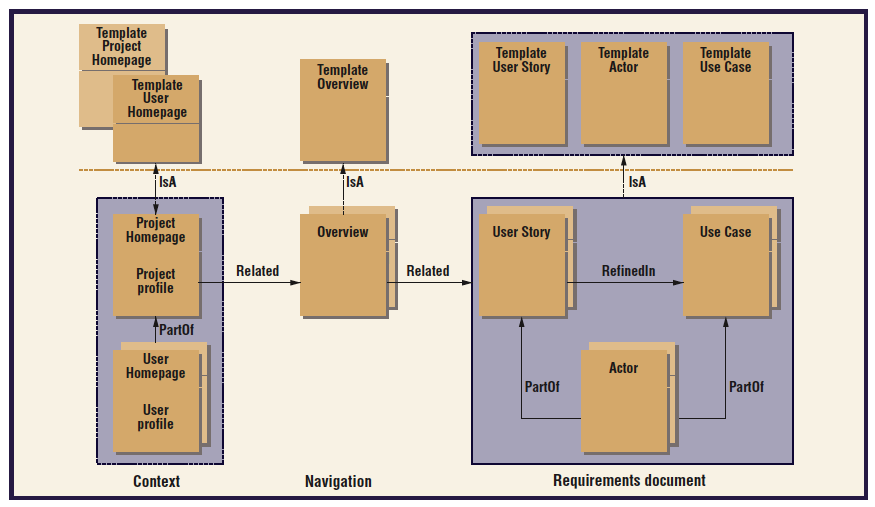
\includegraphics[width=\textwidth]{Wiki.png}
    \caption{A Wiki-Based Document Structure for Requirements Engineering. Source: \cite{wiki_based}}
	\label{fig:wiki}
\end{figure*}

Decker et al. also propose the use of semantic wiki, an approach where additional meta information is used, so that it is possible to reuse the contents using machine learning \cite{self_organized}. In this regard they introduced ``Wikitology'', a term that combines Wiki and Ontology. The Ontology is contained as a part of meta-data in the templates for different software engineering artifacts, such as user stories, discussions, and the like. Once these templates are defined, a software engineering artifact becomes an instance of one of the templates. So, the relationship between two different wiki pages can be established based on their underlying templates' meta information. Given the ontology of different wiki pages, they used two techniques, Latent Semantic Analysis and Case Based Reasoning, to compute the similarity. In this thesis I use the second technique, CBR, to find similarity between an email and a user story. However, instead of using a predefined ontology, Taggy uses the available meta information or context from an email. Also, Taggy combines the context and text similarity in the computation as opposed to solely relying on the context.

Tosic et al. developed Collaborative Semantic Web Portal Prototype. This tool utilizes wiki platform for collaborative knowledge acquisition to be used in agile project management \cite{collaborative_knowledge}. Their solution added access control to the wiki pages and also several indicators for every page such as number of contributors, the creator and so on. Using this system they observed encouraging results such as teamwork and collaboration, open information flow and the light-weight agile vigilance. 

To ease the authoring of wiki pages, OntoWiki incorporates several interesting techniques \cite{ontowiki}. For example, they present a rich editor with support for real-time search from existing content to reduce the time required to produce an article and cross-link with different pages. Also, to make it collaborative they brought the concept of commenting and rating. While these techniques can greatly help in authoring wiki content, to be used in software knowledge management the developers and the customer need to actually put content on the wiki and ensure the content is updated accordingly. This may be a barrier, as it requires dedicating considerable human effort to a cause that has lower immediate business value compared to other tasks, such as developing and testing the software.

Chau et al. studied the contribution to a software wiki made by people working on different roles \cite{a_case_study_of_wiki}. They observed the use of MASE, a wiki-based knowledge sharing system, in a medium-sized software company. They discovered a very high usage of MASE (that exceeds 90\%) as an asynchronous collaboration medium. But surprisingly, only 10\% of the wiki content were produced by the managers, while the rest was contributed by the technical team. Moreover, none of the managers were in the list of top 10 contributors. They also found that there was a greater need for unstructured than structured knowledge. In agile software engineering, informal and continuous customer collaboration is heavily utilized. So, it is important to choose a knowledge sharing media that offers flexibility without a steep learning curve for the customers. This thesis recognizes the need for unstructured knowledge and uses email as a source of such knowledge. As a result, the knowledge base is generated while people communicate as opposed to documented after the knowledge is shared.

Wiki has also been used to write executable acceptance tests with the motivation that customers can provide the acceptance criteria for a user story in simple wiki tables \cite{fitnesse}. For example, Young et al. mentioned the use of wiki for automated acceptance tests so that the continuous integration system could execute the tests \cite{how_did_we}. FIT is a wiki based acceptance testing framework. Melnik et al. found that using a structured acceptance test specification makes it difficult to include irrelevant information in requirement specification \cite{suitability_of}. They also found that acceptance tests using FIT can be easily understood and implemented by a developer with little background about FIT. Such test fixtures are often specified in terms of wiki tables where a set of inputs and their expected outputs are mentioned that can be automatically tested. However, for a distributed team, the acceptance criteria may often be discussed via emails or instant messages. So, if it is possible to see the discussion related to a user story, one can use this as a reference for writing and understanding acceptance test wikis. 

While wiki can work as a knowledge sharing tool, the addition of email discussions offer several unique benefits. First, email is a general purpose communication tool, so most people are already familiar with this. Wikis are great for collaborative editing, but knowledge sharing often takes the form of discussion where information flows back and forth between people. For example, it is easier to follow a discussion than to find the latest changes to a  wiki page. As Chau et al. pointed, wikis and similar centralized knowledge capturing approaches often employ people who are not involved in the day-to-day software development and, as a result, there are concerns raised about the usefulness of this approach\cite{a_case_study_of_wiki}. Capturing knowledge from emails and linking it to user stories will complement the collaborative editing benefits of wiki. So, it will add the useful details that are already discussed from emails to any knowledge from the wikis.

\section{Context-Based Knowledge Management}
Maalej et al. provided a context-based solution for lightweight knowledge sharing in distributed software projects \cite{a_lightweight}. They identified two key steps in the knowledge sharing process, namely, knowledge access and knowledge sharing. They outlined a framework to facilitate the access to relevant implicit knowledge from a large amount of dispersed sources. The framework relies on the context of different knowledge items, as well as knowledge consumer's usage pattern, to proactively provide access to the available knowledge. To facilitate knowledge sharing, they identified that a knowledge provider needs to present the knowledge in generalized format so that it can be applied on a different context by another person. This requires additional effort from the provider without much immediate benefit.

To minimize this burden, they proposed the use of additional semantic information or an additional ontology of knowledge items which can be used in computer-based information retrieval through context matching. Their proposed knowledge management solution derives a profile of the developers from their usage history. Based on this profile and the semantic information present at the knowledge artifacts, the relevant ones are found. This proposed solution mainly targets the knowledge capturing at a fragment of source code level. Although this framework provides an abstract form for a knowledge management solution, a concrete description of how the acquisition of dispersed knowledge from sources like emails, wiki, instant messages and forums are incorporated is not discussed. As suggested in this approach, Taggy uses the context information in addition to text relevance to interlink different knowledge items. However, Taggy is designed to capture high level knowledge from emails and user stories as opposed to the level of source code fragments.

Ratanotayanon et al. developed Zelda, an Integrated Development Environment (IDE) plugin to interlink source code with user stories \cite{supporting_program}. This plugin provides an interface where a developer can select one of the user stories as an active user story. Next, when she is ready to push the changes in the code repository, the plugin automatically links all the changes against the active user story. It also allows a developer to manually select source code that is related to the user story. The goal of this link recording is to help other developers who might need to make changes to the feature from an existing user story. To complete a future modification, one can navigate to relevant source code from the stored links. Since it is a common practice to modify source code and keep revisions, Zelda updates the user story and code links whenever the code has a new revision to keep the links pointed to the latest revision. In their evaluation, they found that Zelda helped developers to focus on relevant source files given a new user story to modify an existing one.

\afterpage{\clearpage}
\begin{figure*}[!htb]
	\centering
	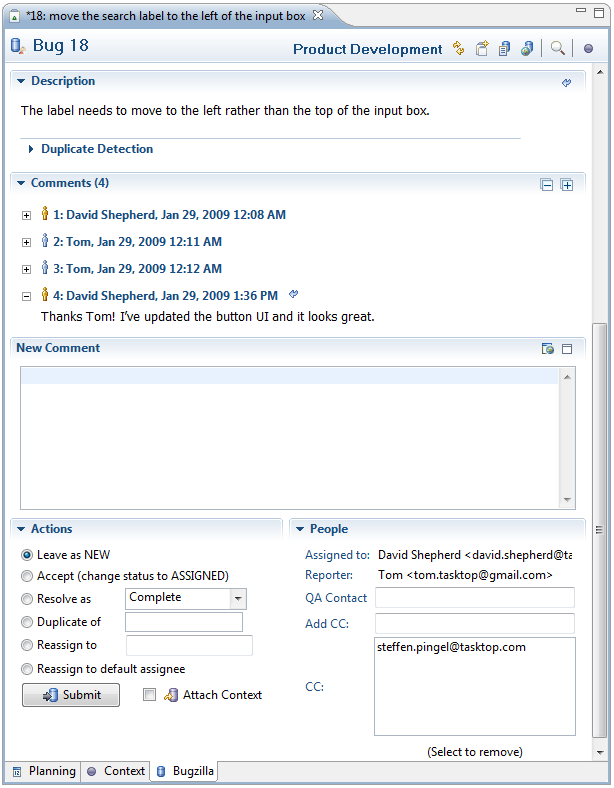
\includegraphics[width=\textwidth]{Mylyn-comment.png}
    \caption{Mylyn Eclipse Plugin - Bugzilla Integration. Source: \cite{mylyn}}
	\label{fig:mylyn-comment}
\end{figure*}

The concept behind Zelda, linking source code changes with requirements and other high level artifacts, is also present in FEAT\cite{feat} and Mylyn\cite{mylyn}. For example, Mylyn is an IDE plugin that builds a task context as developers select a task and make necessary changes. The context of a task includes information about the source code changes, API usage and documentation lookup as a developer works on it. Having this context, a developer can easily navigate and search though relevant source code for a task. Mylyn also has integrations with several task and bug tracking tools. Figure~\ref{fig:mylyn-comment} shows a screenshot of Mylyn where a developer can directly put comments on tasks and browse work items within the IDE while making code changes. Also, they can provide the source context against tasks so that it is possible to locate the source code for a given task as shown in Figure~\ref{fig:mylyn-context}.

\begin{figure*}[!ht]
	\centering
	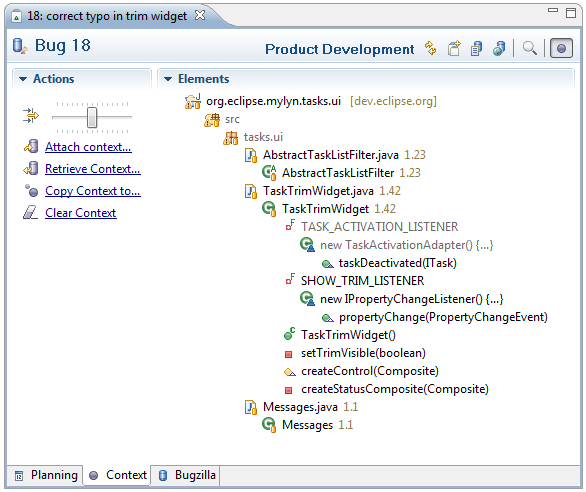
\includegraphics[width=\textwidth]{Mylyn-context.png}
    \caption{Mylyn Eclipse Plugin - Setting source code context of a bug. Source: \cite{mylyn}}
	\label{fig:mylyn-context}
\end{figure*}


As seen with Zelda and Mylyn, high level artifacts such as user stories and tasks can be used as an entry point to a knowledge base. Taggy follows this same approach. However, instead of linking source code with user stories, Taggy links email discussions. So, the knowledge base produced by Taggy is likely to complement Zelda with relevant higher-level information from emails that can provide greater insight into user stories. In a sense, Taggy interlinks two high level artifacts, which complements the knowledge found from interlinked low level items.

\section{Review of Existing Tool Support for Knowledge Sharing}
Distributed agile projects often use globally available project management tools to share knowledge \cite{essential_communication}. These tools allow the teams to capture the product and iteration backlogs, user stories and project planning information. Typical project planning information includes the estimation and assignment of tasks or user stories to developers and testers. Also, some tools provide support for collaboration about the user stories.

\begin{figure*}[!ht]
	\centering
	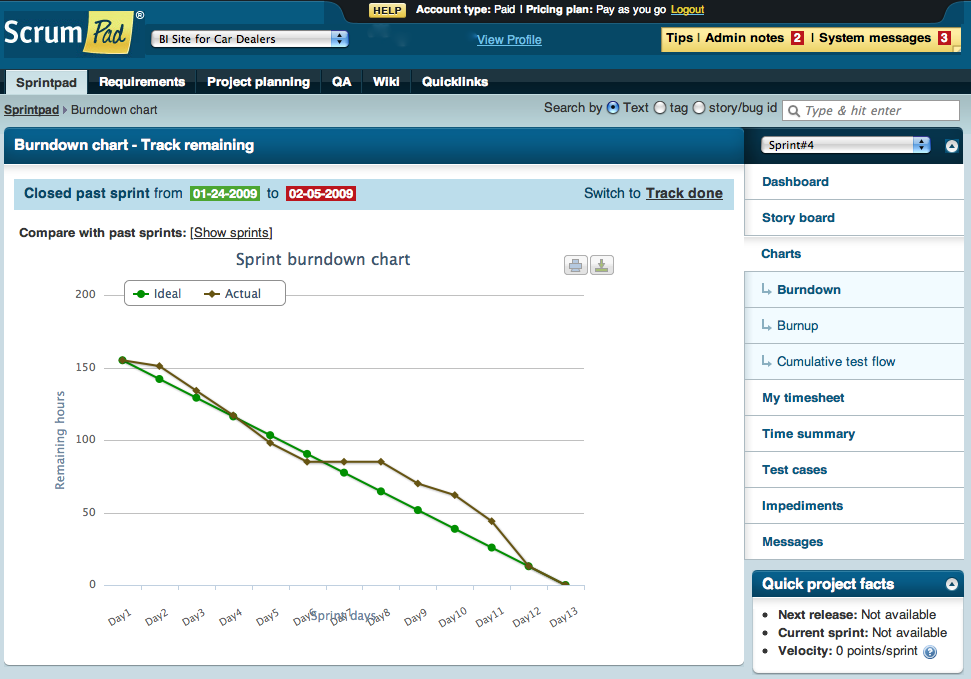
\includegraphics[width=\textwidth]{Scrumpad.png}
    \caption{Dashboard in ScrumPad, a Commercial Agile Project Management Tool. Source: \cite{scrum_pad}}
	\label{fig:scrumpad}
\end{figure*}


There are a number of commercial tools available for agile project management, such as VersionOne\cite{version_one}, Mingle\cite{mingle}, ScrumPad\cite{scrum_pad}, ScrumWorks\cite{scrum_works} and IBM Rational Team Concert\cite{ibm_rtc}. These tools offer templates for capturing various agile software engineering artifacts such as user stories, backlogs, and acceptance tests. Also, they provide process-specific workflows; for example, a workflow for Scrum includes a virtual story wall and various charts for distributed project tracking. Figure~\ref{fig:scrumpad} shows a screen from ScrumPad. As this screen shows, it is possible to search and browse user stories, messages, wikis, etc. as well as produce visual reports on the project's progress using these tools. Some of these tools let people collaborate using message threads and wiki. These tools are generally useful in planning and tracking activities. In addition to commercial tools, one can also use open-source agile project management tools such as XPlanner\cite{xplanner} and Trac\cite{trac}.

Several issue or bug tracking tools such as Jira\cite{jira}, Bugzilla\cite{bugzilla}, and FogBugz\cite{fog_bugz} are being used in distributed agile projects as well. To support agile processes, these tools offer plugins for agile projects that include some of the features from the aforementioned project management tools. These bug tracking tools provide a messaging system where people can collaborate around bugs. The knowledge shared during this collaboration is often used to solve new bugs\cite{issue_tracking}.

Distributed agile teams often use general purpose project management tools such as Basecamp\cite{basecamp} and Teambox\cite{team_box}. While these tools are not tailored to provide agile-specific artifacts, they are often picked for their simplicity of use. So, instead of providing a template for an user story or an issue, these tools simply provide a to-do list. Similarly, instead of iterations, people rely on milestones. And as seen with other tools, the general purpose web-based project management tools also allow people to use messaging systems to collaborate on their to-do lists.

Alongside project management tools, some distributed agile teams use general purpose shareware tools such as Microsoft SharePoint\cite{share_point}. SharePoint provides an infrastructure for managing websites, communities, content, search and reporting that is mainly configuration-based and does not require coding effort for the most part. In large distributed agile projects, where multiple teams are involved, SharePoint is often used to manage the knowledge.

Some agile projects are now using source code hosting platforms for project management as well. For example, github\cite{github}, CodePlex\cite{codeplex} and similar source code hosting platforms have support for defining issues and user stories. Also, they allow some project planning features, such as iteration backlogs, estimation and assignment of work items.

Agile teams also use tools that support continuous integration such as Hudson \cite{Hudson}, CruiseControl\cite{cruise_control} and Microsoft Team Server\cite{team_server} so that the status of the current build is automatically communicated. These tools provide a dashboard and detail view of a project's health that includes build stats, test results and commit history. However, distributed agile teams often use a separate tool to capture knowledge about the high level artifacts that are not found in the continuous integration tools.

The aforementioned tools help distributed agile teams to collaborate and share project-related knowledge. Almost all of them send out notification emails when a change takes place, for example, when a user story is assigned or a build succeeds. Such email notification is helpful since it reaches the inbox of people instead of waiting for them to visit the tools. Some of the tools, such as Basecamp and FogBugz, also accept incoming emails from people. But none of the the tools interlinks the incoming emails to the user stories unless a user does it manually. As a result, the benefits of a message thread attached to a user story is not readily available. To ensure the message threads are kept attached to the user stories, the users are forced to use the tools. But, similar to email notification, this could be convenient if a developer or a customer could just send an email to the tool and the tool would automatically attach the email to the relevant user story. Taggy attempts to solve this problem by utilizing the planning information from the project management tools to infer the relevance of an user story against an email.

\section{Summary}
To summarize, the following key points are found from the related work:
\begin{enumerate}
	\item Distributed teams commonly use emails and instant messages for knowledge sharing. Other popular mediums include wikis, project management tools and continuous integration dashboards etc.
	\item A shared project knowledge base needs to capture and serve useful knowledge from different sources without introducing much human effort.
	\item It is important to build a web of knowledge that connects different software engineering artifacts such as user stories, emails, source code changes and wiki pages so that one can use all available information when needed.
	\item Both the customers and technical team contributes to the knowledge about an agile project. So, a knowledge base needs to allow the flexibly to its end users so that they can utilize their familiar communication mediums.
	\item The context of an artifact can be used to relate it with other artifacts. Also, one can browse the content in a knowledge base starting from an artifact and then following the other relevant artifacts for its given context.
\end{enumerate}
These key points contribute to the requirements for Taggy. Taggy shows a novel technique for knowledge acquisition and tagging from emails and instant messages so that the end users can conveniently contribute without spending any significant effort.


%!TEX root = /Users/smsohan/Taggy/Thesis/ucalgthes1_root_0.tex
\fancyhead[RO,LE]{\thepage}
\fancyfoot{} 
\chapter{Taggy}
\label{ch:taggy}
In this chapter, I have presented the details of my auto-tagging technique in terms of Taggy. Taggy is a prototype implementation of the technique. First, the underlying assumptions behind Taggy are discussed. Then, a definition of the adapted agile project context is given. With this background information, a high level architecture of Taggy is explained. Next, the workflow of auto-tagging is discussed. The mathematical and algorithmic details are provided in the similarity computation section. This chapter also includes the details about the software frameworks used to implement Taggy. Finally, an illustrative example is given to explain Taggy in action.

\section{Assumptions}
Taggy is designed to auto-tag the emails with user stories based on the following assumptions:

\begin{enumerate}
	\item An email is potentially relevant to a user story when:
		\begin{itemize}
			\item It is sent during the iteration time frame of the user story. Since agile projects are developed in small iterations and the core concentration during an iteration is to deliver the user stories from the iteration backlog, it is highly likely that the email conversation will be about the user stories from current iteration backlog. However, it is also possible to see some conversations about near past or near future iteration backlogs. Such conversation are mainly used to provide post-delivery feedback and collaborate about upcoming work. Taggy uses this assumption to shorten its search space for relevant user stories by filtering out the ones from long ago.
			
			\item The developers and/or customers of a user story often communicate via email. For an example, if Alex (a developer) is working on a user story for Jane (the customer), and Alex writes an email to Jane, they are more likely to discuss about the user story than Peri (another developer) and Jane. However, Peri can always participate in a discussion about Alex's work in an agile team, where open communication is encouraged. But, it is highly unlikely that two people who are neither assigned developers or customers of a user story will write emails about that. This assumption about people's participation in email provides an important clue for Taggy's similarity computation.
			
			\item There is a minimum degree of text similarity between an email and a user story. An email has text in terms of its subject, body and attachments. Although not explicit, it is likely that such text in the emails will show some relevance to the user stories. This may not be true in all cases, especially if there is a lot of face-to-face communication. However, this is not the case for distributed projects with huge time zone difference. Taggy computes a text similarity between the email and user story and discards the ones that show very poor match.
		\end{itemize}
	 \item A web-based project management tool is used to manage the distributed agile project. To automatically link up emails with user stories, Taggy looks into this tool for information about user stories. This assumption is required because if teams only use volatile physical artifacts, such as sticky notes for user stories on a whiteboard, it is not possible to automatically find the user stories. As discussed in Chapter~\ref{literature_review}, distributed agile teams use a number of different types of such tools.
	
	\item The project management tool captures user stories with its planning information including a) assigned developers, b) customer and c) iteration timeframe. The presence of this planning information is essential as it serves as the meta data that is necessary to auto-tag emails. While it is generally expected that this data be available, it is not required that each and every user story contains all the required planning information. Since Taggy uses context alongside text similarity, having the context helps in making a more informed decision in auto-tagging.
	
	\item Each project has its own email address termed as ``project email'' so that when people are sending emails about a project to someone, they can keep the project's email in the copy. This serves as the input to Taggy for auto-tagging. Also, giving every project a unique email address ensures Taggy can correctly determine the target project for an email. Since most people who use email are already familiar with the CC: feature, this adds little learning curve or communication overhead. It is assumed that indicating the project in CC: serves a convenient input mechanism compared to manually copy-pasting the email contents into a system for every useful email.		
	
	\item The subject of an email carries an important clue about its relationship with a user story. Although, subject line is just text, similar to the body or attachment contents of an email, due to professional etiquette and for the sake of grabbing attention, people write informative subjects when writing emails about projects. Taggy distinguishes the text relevance of the subject from the rest of the email contents based on this assumption.
\end{enumerate}



\section{The Agile Project Context}
Taggy uses two kinds of context information that are available for agile user stories, namely Temporal context and People context. These contexts are defined below:

\begin{enumerate}
	\item \textbf{Temporal Context.} User stories in agile projects are grouped by small iterations so that a bunch of new user stories are potentially shippable at the end of each iteration. These iterations are confined within specific start and end dates. This time-box works as the temporal context for a user story. For example, if a user story is developed during Iteration\#2, June 1 to June 14, then Taggy assumes people are more likely to write emails about the user story within this period than in the far past or future.
	
	\item \textbf{People context.} The people context for a user story is formed by its assigned developers and customers. A user story may have one or more customers who are mainly responsible for providing the details proactively and as questions arise during implementation. On the other hand, a user story is broken down into tasks and assigned to developers, testers and other technical team members. Taggy uses all the people relevant to a user story as its people context. For example, if an email is exchanged among the people in a user story, then Taggy puts a higher similarity rank than when the people context is different. The identification of the people context is done based on email addresses.
\end{enumerate}

Since Taggy combines context similarity with text similarity, the above contexts provide more information for auto-tagging. However, when some or all of the context information are missing for a user story, Taggy still applies whatever information is available to auto-tag emails with user stories.

\section{High Level Workflow}
Now that the assumptions and definitions of important terms are discussed, Figure~\ref{fig:} shows the two main steps involved in the process of auto-tagging an email with user stories. As with most other machine learning techniques, Taggy needs to learn its parameters concerning relative weights of similarity measures before making decisions. Once learning is done, Taggy uses the learned parameters to auto-tag emails.

%TODO: figure with description
As seen on Figure~\ref{fig:}, the learning process involves several iterations. Since the similarity computation uses multiple components, the learning process needs to address the importance of each component relative to others. To achieve this, first it produces an initial weight for the components and then learns the relative weights based on the training data. The details about learning is discussed later in Section~\ref{sec:learning}.

Once learned, Taggy can be used to auto-tag emails with user stories. This process is designed to be used in a live system as illustrated in Figure~\ref{fig:workflow}
%TODO: figure with description

The details of the auto-tagging workflow as shown in Figure~\ref{fig:workflow} is discussed next:

\begin{enumerate}
	\item \textbf{Copy emails to project mail address.} This is the input step for Taggy. As discussed in the assumptions, Taggy identifies each project by its own email address. So, whenever someone sends an email about a project, they put the ``project email'' in the CC:. This is the only change in the business process that needs to be implemented by the distributed team. This intake process was successfully adapted in previous work \cite{where_did_you}. In case someone forgets to do this while sending the email, it is possible to simply forward the email to the ``project email'' later.
	
	\item \textbf{Grab email.} Once the project related emails reach the inbox of ``project email'', Taggy picks up the email. It is common for email servers to allow access via POP or IMAP protocol. Taggy uses POP3 to read all incoming emails, including the attachments, if any. This grabbing runs on a background process, which can be scheduled to check for new emails in desired intervals. However, this email-grabbing step can make use of any other email transfer protocol.

	\item \textbf{Save email.} After grabbing, Taggy saves the email into its database, keeping a link to its project. After this step, even if auto-tagging fails, the email is still stored under the project. This step makes an email available for search and browsing without the need for looking into other users' inboxes.
	
	\item \textbf{Filter.} To auto-tag the email just grabbed, Taggy first reduces its search space by discarding the user stories of a project that were done in the far past or scheduled to be developed in the far future. This filtering process essentially finds the current iteration of the project, if any. Then, it considers the user stories from the current iteration and its neighboring iterations as potential candidates for auto-tagging the emails.

	\item \textbf{Compute local similarity.} In the reduced search space, Taggy computes local similarities for people and temporal contexts as well as separate text similarities for subject and body. The details of these local similarity computations are discussed in Section~\ref{sec:equations}.
	
	\item \textbf{Compute global similarity.} Next, for each of the user stories, the similarity values from previous step are combined to produce a global similarity score. This computation is done based on the formula presented at equation x. This global similarity assigns a numeric value of the relative relevance between a user story and the email.
	
	\item \textbf{Sort.} The user stories are then sorted descendingly according to their global similarity value from previous step. This produces a list of user stories with the potentially most relevant user story at the top.
	
	\item \textbf{Pick.} Next, Taggy picks the user stories having global similarity scores above a predefined threshold. Having a threshold ensures Taggy only picks the ones that show sufficient relevance based on its learning. However, this also means that for some emails no user story may be picked. Instead of picking up all the user stories above threshold, Taggy can be configured to pick up only the top n stories, where n is a number greater than or equal to one. This allows Taggy to limit the auto-tagging to a limited number of user stories per email.
	
	\item \textbf{Auto-tag.}	Finally, Taggy auto-tags the email with the picked user stories from the last step. This step adds database level links between the email and the user stories to be auto-tagged.
\end{enumerate}

However, to auto-tag instant messages, the first three of the aforementioned steps differ significantly. The following three steps are used for the intake process of instant messages:

\begin{enumerate}
	\item \textbf{Activate instant message plugin.} Instant message clients often allow the use of plugins. For example, Skype \cite{skype} has a plugin framework and Taggy has a plugin for Skype. To input the instant messages, one needs to activate the Taggy plugin and select the project under discussion. Then, as the chat messages are exchanged, the plugin sends out the messages to Taggy over a web-based service. Typically the instant message clients provide meta data such as unique identification of a chat session, its individual messages, people involved and also the time stamp.

	\item \textbf{Grab instant message.} Taggy exposes a web service for the intake of instant messages. As soon as it finds a chat message from the plugin, it identifies the conversation based on the meta data.
	
	\item \textbf{Save instant message.} Taggy extracts out the context from an instant message and saves it in the database. For example, it matches the instant message identifier for people that are already stored in the database against the ones participating in a chat session. Also, it keeps track of the time stamp. As a result, an instant message is stored with a similar people and temporal context as that of an email. Instant messages that are part of a single conversation are stored together in Taggy. The conversation is identified by the supplied identifier from instant messaging client.
\end{enumerate}

Since instant messages don't capture any subject, Taggy cannot produce a subject similarity. As a work around for this limitation, Taggy can be trained differently for instant messages where the contribution of subject similarity is ignored.

On a live system, as like any other machine learning solution, Taggy cannot discard the possibility of a wrong auto-tagging decision. When someone spots such a faulty auto-tagging in Taggy, she/he can manually correct it.

\section{Architecture}
Taggy is composed of a number of different components to support the workflow as outlined in the previous section. The architecture of Taggy is depicted at Figure~\ref{fig:architecture}. Next, the details about each component from the figure is discussed following a bottom-up approach.

\begin{figure*}[bt]
	\centering
	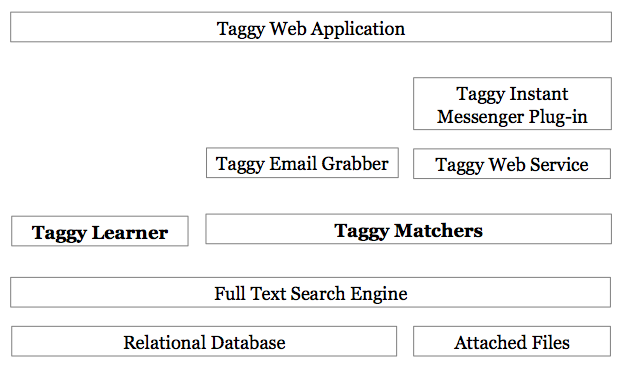
\includegraphics[width=\textwidth]{Architecture.png}
    \caption{Taggy Components}
	\label{fig:architecture}
\end{figure*}

\begin{enumerate}
	\item \textbf{Relational Database.} This relational database component persists the agile project related information. To address the concern of auto-tagging, this database keeps the following information:
		\begin{itemize}
			\item People. People information includes a person's name, email address and instant messenger id, if any. Also, a project vs. people mapping is stored.
			\item Iteration. Iterations, defined by start and end dates, are also saved.
			\item User story. Each user story may have a title and description. Also, if the story is planned, then information about its iteration and assigned people are stored in the database.
			\item Email. The database also stores the subject and content of the emails with a link to sender and recipients if they are found in the people information. If the email is tagged with a user story, then this information is kept in the database as well.
			\item Instant Message. Similar to emails, the database stores the instant messages and their tagging information.
		\end{itemize}

	 \item \textbf{Attached Files.} Attached Files is a simple file system storage where all attachments are kept. An attachment may be part of a user story definition or can be extracted from an email.
	
	 \item \textbf{Full Text Search Engine.} This component produces full text index from contents found in user stories, emails and their associated attachments. This is a third party component that can handle synonyms and language specific stems. The attached files are only indexed for full text search if it would be meaningful - for example, image files are not indexed where PDF file contents are.
	
	\item \textbf{Taggy Matchers.} This is the core component of Taggy that produces the auto-tagging, i.e. the similarity related computations are done inside this component. There are two matchers inside Taggy: email matcher and instant message matcher. These two matchers share some common computation logic. However, instant messages don't have subjects as found in emails and as a result, the two matchers use different relative weights and minimum threshold similarity scores to auto-tag. The matchers depend on the full text search engine and the relational database to lookup required data.
	
	\item \textbf{Taggy Learner.} As discussed before, Taggy requires training to learn different parameters. This component takes care of the learning process. During learning the Learner uses the Matcher to auto-tag an email and depending on the outcome, it may learn the parameters of interest. Once the learning is complete, the learner sets the relative weights to be used in the Matcher. So, the core part of auto-tagger is a mix of its Learner and Matcher components.
	
	\item \textbf{Taggy Email Grabber.} The Email Grabber component works as a background process that periodically checks for incoming emails in any of the project emails. If it finds one, it reads the email, saves a copy in the relational database as well as downloads the attachments into Attached Files. Next, the text contents are all indexed through the Full Text Search Engine. With this data persisted, it invokes the Matcher component to auto-tag the email against the relevant user stories. This handles the email intake process to Taggy.
	
	\item \textbf{Taggy Web Service.} Taggy exposes a web service so that an instant messenger plugin can push instant messages to Taggy.
	
	\item \textbf{Taggy Instant Messenger Plug-in.} This component is installed as a plug in to an instant messenger. Once activated, this component sends instant messages to the Web Service Component.
	
	\item \textbf{Taggy Web Application.} The web application provides interfaces for manipulating everything in Taggy. For example, one can browse a user story and see all related emails and instant messages or vice versa. Also, one can search through all the contents, including the attachments. In a nutshell, this is a light-weight agile project management tool with the additional feature that it auto-tags emails and instant messages.
\end{enumerate}

\section{Similarity Computation}
As I have discussed, the Learner and Matchers are the core component of Taggy. A similarity computation technique forms the heart of these components. In case of Taggy, this is a machine learning technique called Case Based Reasoning (CBR). CBR is used to find out relevant user stories for an email or instant message. 

\begin{figure*}[bt]
	\centering
	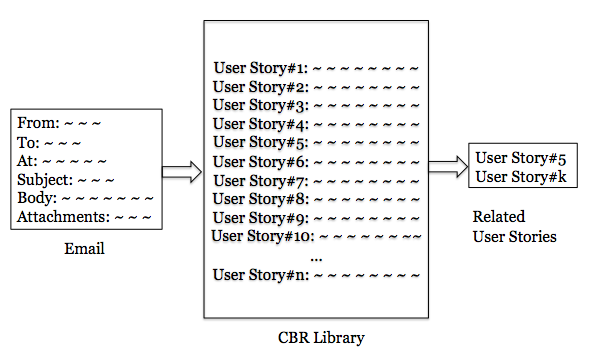
\includegraphics[width=0.8\textwidth]{CBR.png}
    \caption{CBR System Input and Output}
	\label{fig:CBR}
\end{figure*}

Figure~\ref{fig:CBR} shows a high level view of the CBR system. A CBR system uses a library of existing cases to match against a new case. For example, Taggy has a library of existing user stories which are treated as existing cases in the CBR system. Each case is a user story, as described above, is defined by several attributes, such as, its title, description, assigned developers, customers, iteration start date and end date. Also, the data types of the attributes are different in that they include numeric date time values, symbols for emails and free text values. This library of cases is not exactly similar to a new case, an email, since the attributes are different. However, it has been discussed that it is possible to match some of the email attributes against the user story attributes. This action is performed inside the CBR system of Taggy to compute the similarity.


\subsection{Local-Global Principle}

The actual computation inside the CBR system is done following the local-global principle\cite{local_global} where it takes a two step approach, i)local similarity computation and ii) global similarity computation. Local similarity computation is confined to the similarity between only one attribute of two entities. For example, here a local similarity may be the similarity between the date of an email and the iteration start date of the user story. These local similarities are calculated in isolation from the rest of the attributes. So, the local similarity of email date and user story start date is not impacted by their local similarity for people, subject or description.

\begin{table}[at]
  \centering
  \caption{Mapping Between Email and User Story Attributes}
    \begin{tabular}{|p{2.5cm}|p{4cm}|p{5cm}|p{2cm}|}
      \hline
      \textbf{Local Similarity} & \textbf{Email} & \textbf{User Story} & \textbf{Type} \\
      \hline
      People & Sender, Recipients & Developer or Customer & Symbol Array\\      
      \hline
      Temporal & Email Date & Iteration start and end date & Numeric Date \\
      \hline
      Subject & Email subject & Title, Description and Attachments & Free text\\
      \hline
      Body & Email Body, attachments & Title, Description and Attachments & Free text\\
      \hline
    \end{tabular}
	\label{tab:mapping}
\end{table}

Table~\ref{tab:mapping} shows the adapted mapping of email attributes to user story attributes. According to this mapping, the people in email are matched against the people in user stories, so no distinction is made between the sender or recipient of an email. Similarly developers and customers of a user story are not distinguished for similarity computation. The temporal similarity again is a result of comparing the email date against a range defined by the start and end date of the iteration. And as it was stated in the assumptions, subject similarity is distinguished from the body similarity to look for important clues in the email subjects. However, in both cases the comparison is done against all the text found in a user story by looking into its title, description and attachments. This is done because the subject or body of the mail can contain similar text to any part of the user story.

For instant messages, this table remains same for all but the Subject similarity row, since a subject is absent in such cases. So, instant message matching requires one less local similarity measure.

On the other hand, global similarity combines the local similarities and produces a single similarity value between two entities. In this case, the global similarity combines the local similarities for people, temporal, subject and body of an email against the appropriate attributes of the user story. The combination is performed using a weighted sum of the local similarities, where the relative weight for each component is learned during the training phase.

\subsection{Similarity Function}
\label{sec:equations}
Using the aforementioned local-global principle, we adapted different equations to compute the local and global similarities as follows:

\begin{equation}
\label{eq:temporal}
S_{Temporal} =
\begin{cases}
1 & \mbox{iteration start} \le \mbox{email date} \le \mbox{iteration end}\\
0 & \mbox{if email date is within the buffer of the story's iteration} \\
-1 & \mbox{else}
\end{cases}
\end{equation}

S\textsubscript{Temporal} in Equation~\ref{eq:temporal} denotes the Temporal local similarity between an email and a user story. This equation can be interpreted as follows: if the email is sent while the user story is in development, during its iteration, then they show highest temporal similarity. However, it is also likely that an email is sent in the near past or near future of an iteration, this nearness is designated by the buffer. This buffer is set to one iteration length. So, if an email is sent in the immediate past or future iteration of a user story, the temporal similarity is supposed to be 0. Finally, a negative score for the rest ensures emails from far past and far future are treated as highly distant in terms of temporal context. This interpretation is in alignment with the provided assumptions.

\begin{equation}
\label{eq:people}
S_{People} =
\begin{cases}
1 & \mbox{email people = user story people}\\
\frac{\# of \; common \; people}{\# of \;user \;story \;people} & \mbox{email people $\cap$ user story people $\neq$ $\emptyset$} \\
-1 & \mbox{else}
\end{cases}
\end{equation}

S\textsubscript{People} in Equation~\ref{eq:people} denotes the People local similarity between an email and a user story. This function can be interpreted as follows: if an email includes all of the people in the user story, it is highly similar in people context. Otherwise if only a few people are common, the similarity is pro-rated accordingly. Please note that, a user story is supposed to have at least one customer or customer's representative in its people context. However, when an email does not include any of the people in the user story, then it is marked as highly distant from the user story in terms of people context. In other words, this equation produces a numeric value of user story people's participation in the emails.

\begin{equation}
\label{eq:subject}
S_{Subject} = [0, 1]\mbox{, Free text similarity score (See below)}\\
\end{equation}

\begin{equation}
\label{eq:body}
S_{Body} = [0, 1]\mbox{, Free text similarity score (See below)}\\
\end{equation}

S\textsubscript{Subject} and S\textsubscript{Body} represents the free text similarity score for the two attributes. The values can be anything between 0 and 1 as shown in Equation~\ref{eq:subject} and Equation~\ref{eq:body}. Computing the textual similarity between two free format texts is in itself a research topic and beyond the scope of this thesis. However, Taggy used an industry standard open-source full text search engine to produce this score. The search engine uses a Vector Space Model \cite{a_vector_space} to compute the similarity between two free text documents. This model first defines the index of a free text document in terms of a vector that captures the frequency and relative weight of each term in the document. Next, an inner product of two such vectors is used to produce their similarity. Also, to compare the similarity of a document against a library of documents, the similarity results are normalized for the length of the documents. This approach is highly scalable since the similarity computation of two different documents is turned into simple vector computation. Also, the generation of the vectors can benefit from using synonyms, stop words and other language specific stems. Very high-traffic applications have used this approach to facilitate full text search. For example, Twitter, a popular micro-blogging site that serves 12000 searches/second, at the time of writing of this thesis is using this search engine \cite{twitter_lucene}.

%http://engineering.twitter.com/2010/10/twitters-new-search-architecture.html                                                       
The choice of the above equations are based on the experience from looking into the data. However, since the software is trained to learn the relative weights of these equations, the impact of these equations are likely to be weight adjusted so that the global similarity computation minimizes the possibility of a wrong decision.

Next, the global similarity function combines the local similarities from the above equations using the following formula:

\begin{equation}
	\label{eq:global}
S_{Global} = \frac{W_{Temporal} * S_{Temporal} + W_{People} * S_{People} + W_{Subject} * S_{Subject} + W_{Body} * S_{Body}} {W_{Temporal} + W_{People} + W_{Subject} + W_{Body}}\\
\end{equation}

where,
\begin{equation}
	\label{eq:w_temporal}	
W_{Temporal} = \mbox{relative weight of temporal similarity}
\end{equation}      

\begin{equation}   
		\label{eq:w_people}
W_{People} = \mbox{relative weight of people similarity}
\end{equation}

\begin{equation}     
		\label{eq:w_subject}
W_{Subject} = \mbox{relative weight of subject similarity}
\end{equation}

\begin{equation}     
		\label{eq:w_body}
W_{Body} = \mbox{relative weight of body similarity}
\end{equation}

As Equation~\ref{eq:global} shows, the global similarity is a weighed sum of the local similarity values. But the relative weights are not known a priori. Instead, Taggy learns the relative weights for the different components so that it can potentially reflect the relative importance of each of the component based on a training data set. Using a weighted sum provides transparency about the decision-making logic inside Taggy.
	
\subsection{Learning Relative Weights}	
\label{sec:learning}
Taggy uses a Reinforcement Learning approach to learn the relative weights of the different components to compute a measure of global similarity \cite{reinforcement_learning}. The learning algorithm is designed to adapt the relative weights of the local similarity measures based on the feedback from its decision being correct or incorrect.

Since the local similarity measures participate in the process of global similarity computation, in case of a correct decision, the matching local similarity measures get rewarded by getting more weight while the contradicting ones are punished by lowering their relative weight. For example, if a decision is correct and the people similarity score is positive, then the relative weight of people similarity score, as seen in Equation~\ref{eq:w_people}, is increased. On the other hand, if the decision is correct but the people similarity score is negative, then it is punished by lowering the weight. So, depending on the decision of an individual component and the final outcome, the relative weights are adjusted accordingly. This process continues unless all training data are exhausted or the adaptation converges.

However, it is important to initialize the relative weights of the local similarity measures based on a meaningful foundation so that the entry point is not absolutely random. This is done by running the training data for each local similarity while keeping the others in isolation - for example, trying to auto-tag emails with user stories solely based on their people similarity and doing the same for other local similarity components. Once this is done, the number of correct decisions made by each component provides a rough estimate of its relative importance over another component. These numbers of correct decisions are normalized to produce the initial relative weights of the four components, namely, people, temporal, subject and body similarity measures.

Once the initial weights are found, the following algorithm is used to implement the reward-punishment scheme of the reinforcement learning approach:

\pagebreak
\begin{verbatim}
date_weight     = initial_date_weight
people_weight   = initial_people_weight
subject_weight  = initial_subject_weight
body_weight     = initial_body_weight

for all_training_emails do |email|
   result = find_most_similar_user_stories(email)
   is_correct = result.guessed_stories == email.actual_stories

	 #Adjust temporal similarity weight
   is_date_similar = result.date_weight > 0

   if (is_correct and is_date_similar) or 
      (!is_correct and !is_date_similar) then
    date_weight = reward(date_weight)
   else
    date_weight = punish(date_weight)
   end

   #do the same for people, subject and body similarity
		. . .
		
   end
end
\end{verbatim}
This algorithm shows the reward-punishment in action for the temporal similarity weight. This essentially rewards the local similarity weight of a component that contributes in making a correct decision while punishes the one that influences a wrong decision. This reward-punishment continues unless all training emails are seen. Also, it is possible to stop if this converges to a point when adding new emails do not alter the relative weights. However, as with most machine learning techniques, the usefulness of this learning is related to the quality and quantity of the training data. As shown before, Taggy's Learners component implements this algorithm. Once the learning is done, relative weights are tuned to auto-tag emails with user stories. This same algorithm can be used to learn relative weights for instant messages, where the subject is missing.

The choice of this reward-punishment scheme makes it transparent, as one can easily follow the changes in the relative weights based on the logic. Other machine learning approaches such as different variations of back propagation algorithm could also be utilized instead of this one. However, this approach was chosen in Taggy since it is a transparent learning approach where one can monitor the changes in relative weights at each step of the learning.

\subsection{Email Matching}
Once the relative weights are learned, Taggy can match emails against user stories based on the trained system. This process essentially starts with grabbing email and saving it. A developer or customer sends out emails about the project and copies to Taggy using CC: feature. While saving, a lookup is performed to see if the email addresses present in the sender, recipients and CC: match against any of the existing users' record in Taggy's relational database for the project. If found, the users are linked with the emails. Next, the email matcher of the Taggy Matchers component is asked to look for relevant user stories in the database.

\begin{figure*}[tb]
	\centering
	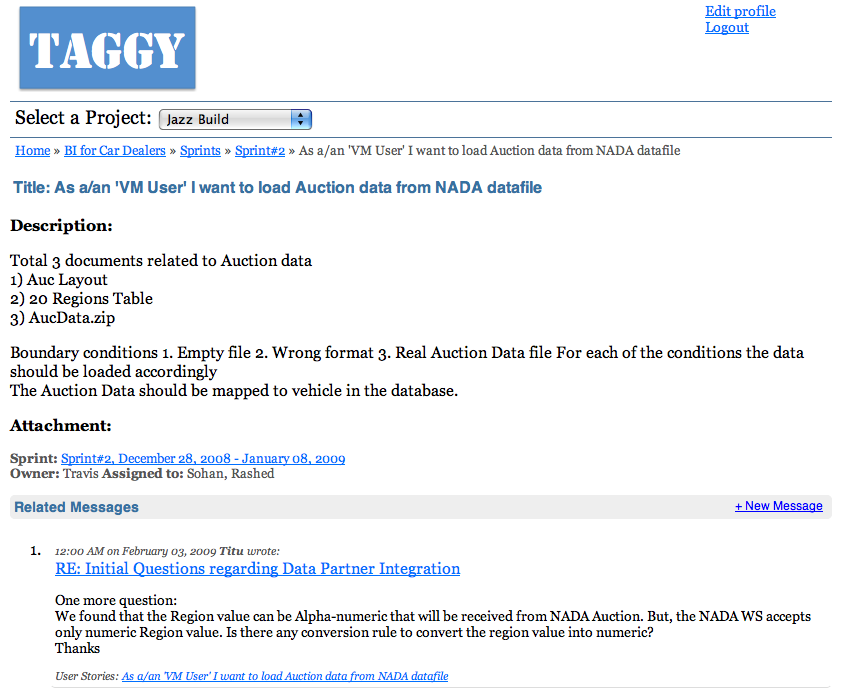
\includegraphics[width=\textwidth]{taggy_user_story.png}
    \caption{Taggy Screenshot - Showing User Story and Related Emails}
	\label{fig:taggy_user_story}
\end{figure*}

\begin{figure*}[tb]
	\centering
	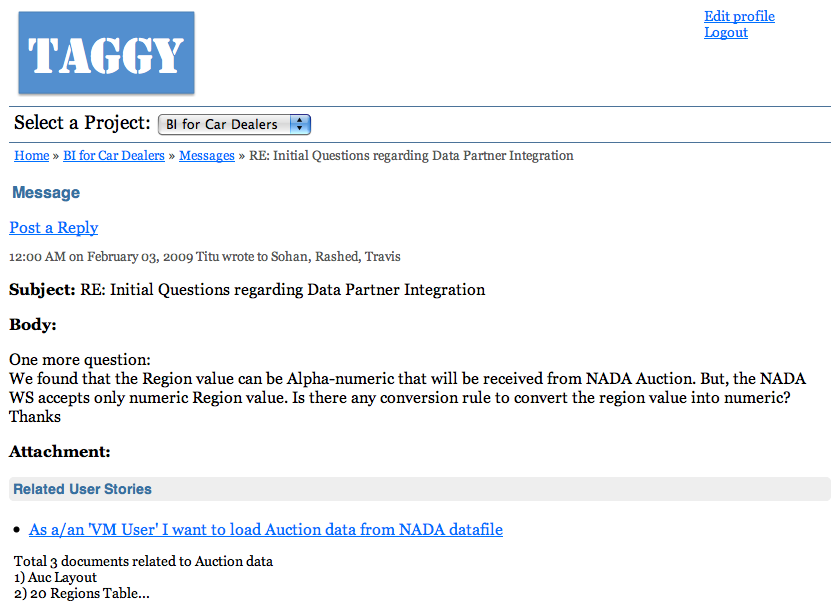
\includegraphics[width=\textwidth]{taggy_email.png}
    \caption{Taggy Screenshot - Showing Email and Related User Stories}
	\label{fig:taggy_email}
\end{figure*}



To an end user of Taggy, the outcome of auto-tagging is as shown in Figure~\ref{fig:taggy_user_story} and Figure~\ref{fig:taggy_email}. So, while browsing user stories, one can see the related emails or vice versa. This same outcome is found for instant messages as well. So, this email matching is responsible for ``matchmaking'' among the emails and user stories based on their context and text similarity.

The email matcher filters out user stories so that user stories from far past or future are discarded. Next, it computes the local similarity measures and combines them  to produce global similarity values. The ones that show a global similarity above a threshold, survives as the potential candidates for auto-tagging. Based on user preferences, the email is auto-tagged against the top n user stories, where n is any number greater than or equal to 1. The following code fragment shows these steps:

\pagebreak              
\begin{verbatim}
def	find_most_similar_user_stories(email, n)
  nearby_user_stories = UserStory.planned_nearby(email.date)

  if nearby_user_stories
    temporal_scores = find_temporal_scores(nearby_user_stories, email.date)
    people_scores 	= find_temporal_scores(nearby_user_stories, email.people)
    subject_scores 	= find_subject_scores(nearby_user_stories, email.subject)
		email_text 			= email.body_with_attachment
    body_scores 		= find_subject_scores(nearby_user_stories, email_text)

    global_scores = compute_global_scores(relative_weights, temporal_scores, 
																people_scores, subject_scores, body_scores)

    global_scores_above_threshold =  discard_under_threshold_scores(global_scores)

    if global_scores_above_threshold
    	return global_scores_above_threshold[0..(n-1)]
    end
		
  end
	
  return blank
	
end
\end{verbatim}

The different similarity computations in the email matcher are carried out using the Equation~\ref{eq:temporal}, Equation~\ref{eq:people}, Equation~\ref{eq:subject}, Equation~\ref{eq:body} and Equation~\ref{eq:global}. As shown in the code fragment, one can configure Taggy email matcher to auto-tag with the top n number of top matches. Having n greater than 1 helps to identify cases when an email is potentially relevant about two or more user stories. However, in some teams this situation may be different where most of the time the communication is just about a single user story. So, this configuration will help them to tune Taggy according to their communication patterns. Although not implemented, Taggy could also learn this parameter, n, based on the training data. If the the training data shows that most emails only discuss a single user story, it may only choose to show the most relevant story or adjust this number based on the trend.

This matching algorithm is run in the same background process as that of the Email Grabber. Because of the filtering step, Taggy has a reduced search space to deal with. Although this improves speed, it may produce a wrong decision if a distributed agile team chooses to discuss about user stories from the distant past in the emails. In such cases, the definition of ``distant'' needs to be adjusted accordingly. In the implementation of Taggy, anything beyond immediate past and future iteration is treated as ``distant'' based on the observation from training data.

\subsection{Instant Message Matching}
The instant message matcher is implemented using the same approach, since we can find similar people and temporal context from instant messages as well. As discussed earlier, the intake process is different for instant messages, which uses a Taggy web service to push chat messages from a Taggy Instant Messenger Plug-in. The actual similarity computation in case of instant messages omits the subject similarity and applies a different relative weight scheme. The threshold is also adjusted accordingly.

\section{Implementation Details}
Figure~\ref{fig:implementation} shows the implementation frameworks for the different architectural components.


\begin{figure*}[bt]
	\centering
	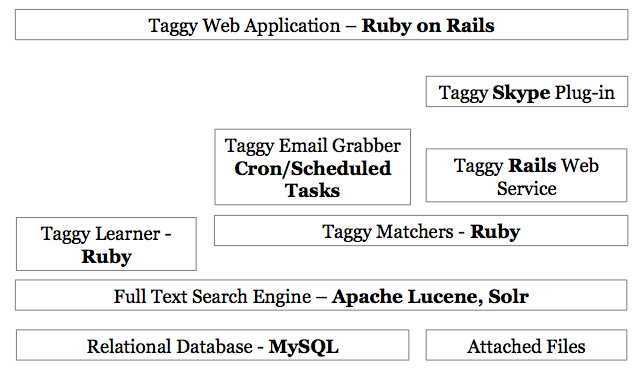
\includegraphics[width=\textwidth]{Implementation.png}
    \caption{Taggy Implementation Details by Component}
	\label{fig:implementation}
\end{figure*}



As with any software solution, the implementation of Taggy was based on available programming languages and platforms. The core Taggy components, the Learner and Matcher, are developed using the Ruby programming language\cite{ruby}. The web application is also developed using the open-source Ruby on Rails web framework \cite{ruby_on_rails}. The choice of this framework was based on my prior experience as well as its support for producing quick data-backed web application development.

The full text search is served by Apache Lucene \cite{lucene}. This open-source search engine is widely used across the web to facilitate full-text search. A previous implementation of Taggy used Microsoft SQL Server Full-Text Search Engine\cite{auto_tagging}\cite{sql_server}. But Lucene was chosen because of its ability to index rich text files such as Word Documents, and PDF files. Also, Lucene can be configured to support synonyms, language stems and comes with out-of-the-box support for full-text search using several languages. However, the architecture of Taggy allows the replacement of this engine by another one without impacting the rest of the system.

To communicate with Lucene, a web service wrapper called Solr is used\cite{solr}. Solr's RESTful web API provides easy access to Solr indexing and querying from other languages, such as Ruby. To handle attachments, a Solr query can include a file and then produce its index similar to other documents based on its content.

Since most project management tools support full-text search anyway, this indexing is not likely an additional burden applied by Taggy. However, Taggy may need to deal with additional contents that originate from emails and instant messages.

For capturing instant messages, a Skype plugin is developed using the Skype4Py library\cite{skype4py}. The plugin can be turned on/off by the click of a button. When activated, it copies the chat messages with meta information and sends this data to the web service. Skype was picked because its use as a popular instant messenger service in software knowledge sharing\cite{how_did_we}. Also, it offers a suite of features that are used by distributed agile teams such as group chat, group video conferencing, and screen sharing. A similar plugin can be developed for other instant message services if supported by the platform.

The background process for the email grabber can be run using Cron jobs on Unix based platforms or scheduled tasks on Windows based platforms \cite{cron} \cite{scheduled_tasks}. These scheduling tools can be configured to look for new incoming emails in preferred intervals starting from once every second to any realistic period.

Taggy used a MySQL relational database server to store the data. This can be replaced by any relational database supported by ActiveRecord, which including MySQL, Oracle, Microsoft SQL Server, SQLite, Derby etc\cite{active_record}. Also, it is possible to use any data storage without using ActiveRecord at all as long as Taggy gets similar data.

As of hardware platform, Taggy does not impose any special requirements compared to other agile project management tools.

\section{An Illustrative Example}	
Now that the details about Taggy's internals are provided, the following illustrative example will demonstrate Taggy in action.

First, a project's backlog is populated with user stories. This backlog has stories from different iterations. For brevity, a shortened backlog is given at Table~\ref{tab:backlog}:

\begin{table}[h!]
  \centering
  \caption{An Example Product Backlog}
    \begin{tabular}{|p{0.5cm}|p{1.7cm}|p{1.2cm}|p{1.2cm}|p{9cm}|}
      \hline
      \textbf{\#} & \textbf{Iteration} & \textbf{Cust- omer} & \textbf{Deve- loper} & \textbf{Description}\\
      \hline
		1 & \#1, Dec 14-25, 2008 & C1 & D1 & As a/an `VM User' I want to add/edit/view dealer account profile so that VM can earn revenue from charging a monthly subscription fee.
			Dealers will have three contacts: Billing, General Manager and Owner. Also, there will be a primary and secondary contact. More information is attached.\\
      \hline
		2 & \#1, Dec 14-25, 2008 & C1 & D2 & As a/an `VM Admin' I want to add/edit/view VM users. 
		Administrator must be able to see username but not password VM Users will be one of inside rep and outside rep. 
		Required fields and more information are attached...\\
	  \hline
		3 & \#2, Dec 28, 2008-Jan 08, 2009 & C1 & D1 & As a/an `VM user' I want to load DMV data from Experian from a CSV/Excel file into VM database. Sample data attached.\\
	  \hline
		4 & Not Assigned & C1 & D1 & As a/an `VM User' I want to activate and deactivate a dealer\\
	  \hline
    \end{tabular}
		\label{tab:backlog}
\end{table}

This backlog has 4 user stories. The stories are assigned to two developers, D1 and D2, and only one customer C1. Also, this backlog contains stories from Iteration\#1, December 14-25, 2008 and Iteration\#2, December 28, 2008 to January 8, 2009. Also, the user story\#4 is not yet planned for any iteration. In an agile team, this list is likely to be longer with more user stories, iterations, developers and customers. However, for the sake of an example, this small backlog serves the purpose.

Now, developer D1 needs to get a clarification from the customer C1 while working on a user story at the start of iteration\#1. This is asked using the email as shown below:

\begin{quote}
	\emph{\textbf{To:} C1}\\
	\emph{\textbf{From:} D1}\\
	\emph{\textbf{CC:} project@Taggy}\\
	\emph{\textbf{Date:} Dec 14, 2008}\\
	\emph{\textbf{Subject:} Initial Questions on \textbf{Dealer setup}}\\
	\emph{\textbf{Body:}\\
	Please clarify the following questions regarding dealer setup data-\\
	1. Is it ok to assume that the billing, GM and Owner contacts of a dealer will also contain username/passwords. Note that, the main and secondary contacts as well as the Used car manager contact contain user name/passwords.\\
	2. What data should we collect for Physical Address and Mailing Address of a dealer? Is it free text? Or collected as fields street1, street2, city, state, zip, country?\\
	3. Is it possible that for a dealer both an inside and outside salesman is assigned?\\
	4. Apart from the name and pricing, is there any other field associated with the ``program'' {main/platinum} information?\\
	5. What is meant by the ``Location'' field of the outside VM Rep?\\
	6. Is it possible to provide us with a sample input data that will be used to set up an inside/outside VM user's commission? Please provide examples of default, bonus, retention and special commissions.\\
	7. What are the required fields of all the dealer setup fields?\\
	8. The Business Address is mentioned twice under the 5.6.1.5 - do we need to capture two business addresses?
	}\\
\end{quote}

Please note that this email has a CC: to project@Taggy. So, Taggy will be able to read the contents of this email. As shown in the email matcher, Taggy will try to auto-tag the email with the existing user stories based on context and text relevance. While doing so, the local and global similarities are computed as shown in Table~\ref{tab:similarity}:

\begin{table}[h!]
  \centering
  \caption{Similarity Scores}
    \begin{tabular}{|p{1.2cm}|p{1.5cm}|p{1.2cm}|p{1.2cm}|p{1.2cm}|p{1.4cm}|p{1.4cm}|p{1.1cm}|p{1.1cm}|p{1.2cm}|}
      	\hline
		\textbf{Story \#} & \textbf{Tempo-ral Sim.} & \textbf{Tempo-ral. Wgt.} & \textbf{People Sim.} & \textbf{People Wgt.} & \textbf{Subject Sim.} &\textbf{Subject Wgt.} & \textbf{Body Sim.} &\textbf{Body Wgt.} &\textbf{Global Sim.}\\
		\hline
		1 & 1 	& \multirow{4}{*}{28.6} & 1 	& \multirow{4}{*}{20.2}	& 0.6 & \multirow{4}{*}{34.4}	& 0.4 & \multirow{4}{*}{16.8}	& \textbf{0.76}\\
		2 & 1 	&  & 0.5 	&  	& 0.4 	&	& 0.25	&	& 0.57\\
		3 & 0 	&  & 1 		& 	& 0 		& & 0.2	&	& 0.24\\
		4 & -1 	&  & 1 		& 	& 0.3 	& & 0.3	&	& 0.07\\
		\hline
	\end{tabular}
	\label{tab:similarity}
\end{table}  

Here, similarity scores are computed based on the similarity equations. For example, user story\#1 has a people similarity score of 1, since all people in the story, C1 and D1, are present in the email. On the other hand, user story\#2 has a people similarity score of 0.5 since only one (C1) of the two people from the user story is found in the email. The values for other similarity measures can also be traced following the respective equations.

From the above table we see that Story \#1 is the most similar story to the given email with a similarity score of 0.76. This is greater than the threshold of 0.58 (details discussed in Chapter~\ref{ch:evaluation}) and thus the system auto-tags the email with Story \#1. However, the other stories are not considered as related as those failed to reach the threshold similarity score.

In this example the email is auto-tagged with user story\#1. However, if the threshold is set to a lower value or there was another user story with similar profile to user story\#1, Taggy could recommend more than one auto-tagging. On the other hand, it could simply ignore auto-tagging with any user story if another email was too irrelevant for the given backlog.

Taggy does not distinguish between a new email and return to an existing email. This is because the return email typically contains the same subject and original email along with the new text in the body. So, whatever decision was applied to the original email is likely to be applied to a return email unless there is a significant change in any or some of people, date, subject or content of the email. In the later case, it is logical that this email indeed is a new one and may be a candidate for completely new auto-tagging with different user stories. This is a design trade-off since identifying return emails and applying the same tags as their original emails would be faster compared to recomputing the auto-tagging. But the auto-tagging is run on a background process. So, the cost of rerunning the auto-tagging is less expensive than following the wrong way in case the previous email had inappropriate auto-tagging or the new reply has significant change compared it is predecessors.


%!TEX root = /Users/smsohan/Taggy/Thesis/ucalgthes1_root_0.tex
\fancyhead[RO,LE]{\thepage}
\fancyfoot{} 
\chapter{Quantitative Evaluation}
\label{ch:evaluation}
As previously mentioned in the research goals, an evaluation is required to measure the accuracy of Taggy in auto-tagging emails with user stories. In this thesis, the evaluation is based on two different real world data sets, collected from two different sources. In total, the data represents 4,745 messages created by 9 agile teams. The evaluation shows that for different projects Taggy can correctly auto-tag between 76\% to 81\% emails with user stories after sufficient training.

This chapter is organized as follows: Firstly, the evaluation approach is discussed. As a part of it, the adapted definition of accuracy is given. Next, a null hypothesis is stated which is used in deducing the statistical relevance of the evaluation results. Then, the two data sets are described and the evaluation results for each are provided in detail. Finally, the limitations of this evaluation are discussed.

\section{Evaluation Methodology}
The evaluation steps, as depicted in Figure~\ref{fig:evaluation}, are described below.

\begin{figure*}[h!]
	\centering
	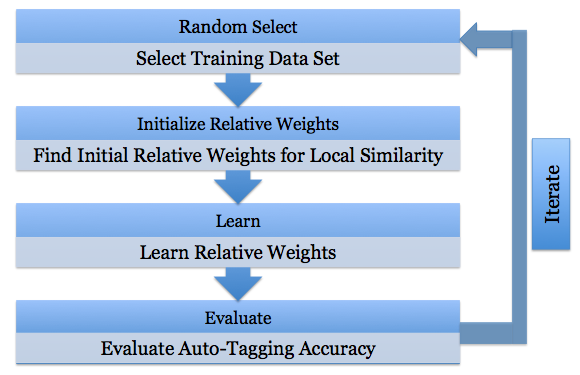
\includegraphics[width=\textwidth]{Evaluation.png}
	\label{fig:evaluation}
  \caption{Taggy Empirical Evaluation Steps}
\end{figure*}


\begin{enumerate}
	\item \textbf{Random Select.} Randomly select 10\% emails from all available emails for training. Training emails are randomly selected to cover the different patterns in the data and eliminate selection bias.
	\item \textbf{Initialize Relative Weights.} Initialize the relative weights for temporal, people, subject and body similarities using the training data from step\# 1.
	\item \textbf{Learn.} Use the reward-punishment approach for each training email from step\# 1, adjust the relative weights.
	\item \textbf{Evaluate.} Using the adjusted relative weights from step\#3, auto-tag the remaining emails that were not included in the training data in step\# 1. This ensures the training data and evaluation data contain completely disjoint sets of emails. Compute the accuracy of the auto-tagging.
	\item \textbf{Iterate.} Repeat steps 1 to 4, with 20\%, 30\%, 40\% and 50\% data for training. This step attempts to find an optimum partition of  training data set where the relative weights converge to a point so that adding more training data adds little value to the auto-tagging accuracy. However, this step is not required for the evaluation only. In practice, Taggy auto-tag emails for any project based on its learning from historical data in existing projects.
	
\end{enumerate}

\subsection{Accuracy}
An auto-tagging is correct if i) it tags with the right user story or ii) does not tag when no relevant user story exists. In other words, it is incorrect if i) it tags with an irrelevant user story or ii) does not tag even though a relevant user story exists. The accuracy of auto-tagging is a ratio between the number of correct tags and the total number of emails presented for evaluation. Since this excludes the training data set, the accuracy only represents the accuracy over the evaluation data set. So, the accuracy is computed using Equation~\ref{eq:accuracy}.
	
\begin{equation}
\label{eq:accuracy}
Accuracy = \frac{Number \;  of  \; correct  \; auto tagging} {Number \;  of \;  total \;  evaluation \;  emails }  \; *  \; 100  \; \%
\end{equation}
	
As Equation~\ref{eq:accuracy} suggests, it is necessary to be able to justify whether an auto-tagging is correct or incorrect. So, the evaluation data needs to provide information about correct relationship of an email with user stories so that the auto-tagged results can be compared against  known values.

\subsection{Statistical Relevance}
The statistical relevance is found by starting with a null hypothesis and then observing the goodness-of-fit of the evaluation data based on chi-square test \cite{chi_square}. In this case the null hypothesis is:

\begin{quote}
	The auto-tagging accuracy of Taggy is no better than a random decision making.
\end{quote}

The outcome of an auto-tagging process is either a correct or a wrong tagging of an email against the user stories in a project. Similarly, a random system will produce one of the two outcomes. The target of this statistical relevance determination is to see if the accuracy found from Taggy's evaluation is better than that of a random system.

In this case, we have a single degree of freedom, since there are two possible outcomes, correct and incorrect. A random system may produce either a correct or incorrect tag for each email. So, the expected value of correct and incorrect tagging for a random system is same, which is half of the total emails. Based on this information, the chi-square computation is done using Equation~\ref{eq:chi}:

\begin{equation}
\label{eq:chi}
\begin{split}
	\chi ^ 2 = \frac {(Count \; of \; correct \; tagging \; - \; half \; of \; total \; evaluation \; emails) ^ 2} {half \;  of \;  total \;  evaluation \;  emails} +  	
\\
	\frac{(Count \; of \; wrong \; tagging \; - \; half \; of \; total \; evaluation \; emails)  ^ 2} {half \; of \; total \; evaluation \; emails}
\end{split}	
\end{equation}                                       

This computed $\chi^{2}$ value is compared against the upper critical chi-square value for probability 0.05 with 1 degree of freedom, that is $\chi^{2}_{0.05}$=3.841. The probability value of 0.05 is conventionally used in significance finding. A value above this threshold indicates disagreement between the observation and the null hypothesis. We also present the corresponding p-values against the computed chi-square values. The lower the p-value, the less likely it is that the observation is true given the null hypothesis holds. For example, a p-value of 0.05 implies the following: there is a 5\% chance of the observed result are by pure chance (i.e. one in 20 studies produce statistically significant results by chance and 19 out of 20 studies are showing that the null hypothesis is incorrect because there is a real causal relationship)

\section{Evaluation Results}
The evaluation results are discussed in two sections for two different data sets.

\subsection{Data set\# 1: ScrumPad}	
This data set was obtained from an online agile project management tool called ScrumPad.	ScrumPad allows users to manage product backlog, perform iteration planning and track progress. Also, it lets users discuss the project's user stories using message threads. Each message thread can contain an explicit link to a user story. While sending a message using ScrumPad, one can link it with a user story. The messages are stored in ScrumPad database and also sent to people via emails. People can directly reply to the notification emails, which goes to ScrumPad and gets saved as a message either in a new or under an existing thread.

The user stories in ScrumPad contain information about its title, description, attachments, customer, developers and iteration. We used these user stories to train and evaluate Taggy's auto-tagging accuracy.

\begin{figure*}[h!]
	\centering
	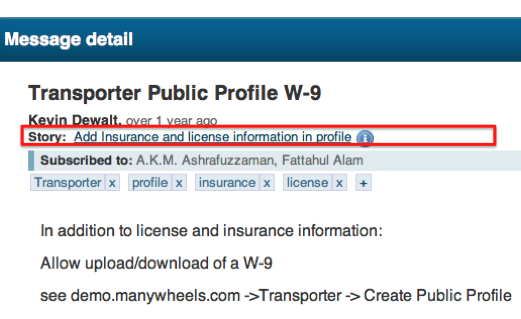
\includegraphics[width=0.8\textwidth]{scrumpad_message.png}
   \caption{A ScrumPad Message Linked to a User Story}
	\label{fig:scrumpad_message}
\end{figure*}

Figure~\ref{fig:scrumpad_message} shows the screenshot of a message at ScrumPad. As this figure shows, the message has a link to the user story. The messages from ScrumPad message threads are derived as emails for the evaluation of Taggy. Messages contain subject, body, sender, recipients and attachments. These fields are mapped against the standard fields of emails. Also, if a message thread in ScrumPad is linked against a user story, all derived emails from the messages of that thread are also treated to be linked against the user story. So, these are essentially the correct tags for the emails since they were all manually provided by the contributors to the message threads. This information helps the training of Taggy using reward-punishment approach with the necessary feedback. Also, the accuracy computation relies on this information to find if an auto-tagging is correct or not.

ScrumPad data set contains data from five distributed agile projects. Four of the five projects, MethodMarketing, BI for Car Dealers, ManyWheels and VarsityDays were developed by Code71, Inc. (www.Code71.com). Code71 is also the creator of ScrumPad. These four projects employed developers from Dhaka, Bangladesh and Virginia, USA. These projects were developed for four different clients from USA.

The fifth project, MindAndMarket, was distributed among one developer from Bangladesh, and two developers and a client from Belgium. The Belgian development team and the client worked at the same city.

\begin{table}[h!]
  \centering
  \caption{Scrumpad Data Set}
	\label{tab:scrumpad_data_set}
    \begin{tabular}{|p{2cm}|p{4cm}|r|p{1cm}|p{1.2cm}|p{1.2cm}|r|}
      \hline
      \textbf{Project Name} & \textbf{Description} & \textbf{Users} & \textbf{Itera- tions} & \textbf{It. Len. (days)}  & \textbf{User Stories} & \textbf{Emails}\\
      \hline
      Method Marketing & Online loan application & 7 & 14 & 14 & 86 & 183 \\
      \hline
      BI for Car Dealers & A decision support tool for vehicle dealers & 7 & 11 & 14 & 70 & 213 \\
      \hline
      Many Wheels & A web application for transporters and shippers & 5 & 12 & 14 & 97 & 158 \\
      \hline
      Varsity Days & A social networking application for school sports teams & 5 & 15 & 14 & 88 & 46 \\
      \hline
      Mind And Market & A project collaboration tool & 3 & 6 & 7 & 28 & 40 \\
      \hline
      \textbf{Total} &  &  &  &  & \textbf{369} & \textbf{640}\\
      \hline
    \end{tabular}
\end{table}

Table~\ref{tab:scrumpad_data_set} shows the composition of this data set. In total, this data set contained 640 emails and 369 user stories from 5 distributed agile projects. It is worth mentioning that 640 messages were exchanged using ScrumPad. However, the actual number of project related emails may not be limited to this volume.

Given this data, the aforementioned evaluation approach was followed to train and auto-tag the emails. The iterative approach resulted in an optimum  training data partition size of 20\% from each project. This size was selected because, from each project, a random partition containing 20\% of the emails for training produced better auto-tagging accuracy than a smaller sized partition (e.g. 10\%) and was as good as a larger sized partition (e.g. 30\%). 

\begin{figure*}[htb]
	\centering
	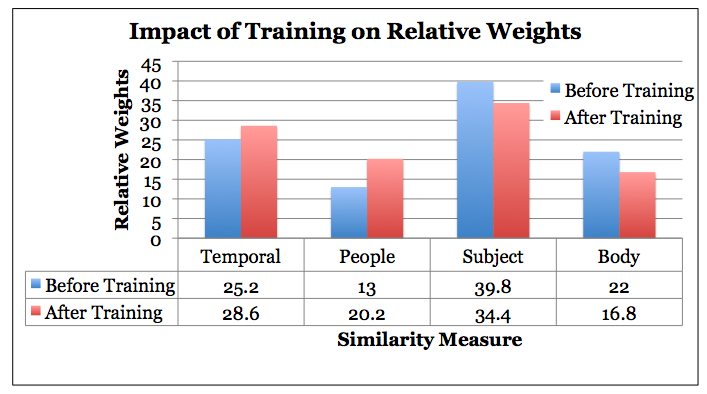
\includegraphics[width=\textwidth]{training.png}
    \caption{Impact of Training on Relative Weights}
	\label{fig:training}
\end{figure*}

Chart~\ref{fig:training} shows the impact of training on the relative weights of different similarity measures. The chart shows that the initial relative weights for the similarity measures of the text components (subject and body) are reduced while the context components (temporal and people) are increased as a result of the training. The initial relative weights were found using the method as discussed in Section~\ref{sec:learning}.

Instead of training Taggy on a per project basis, I used 20\% data from all the projects. As a result, Taggy could benefit from a large number of training emails. However, it is possible to use a per project learning as well. I have discussed the trade-off regarding learning for specific project vs. a collection of projects at Chapter~\ref{ch:discussion}.

The maximum similarity score for a local similarity measure can be 1.0 as shown in the similarity equations at Section~\ref{sec:equations}. For an example, using the trained relative weight values and a threshold global similarity score of 0.58, an email will be auto-tagged with a user story if one of the following is true:
\begin{enumerate}
	\item The email has strong text similarity (maximum 0.34 + 0.17 ~= 0.51) and some context similarity with the user story.
	\item The email has context similarity (maximum 0.29 + 0.20 ~= 0.49) and some text similarity with the user story.
\end{enumerate}
The global similarity function produces the combined similarity value, which is compared against the threshold score. Setting such a threshold score forces auto-tagging decisions to be based on both context and text relevance. This threshold was found from observing the data. In the training data, the global similarity function produced a score of 0.58 or higher for 90\% of the actual email and user story relations. This cut-off point helped to eliminate some false positives. The trade-off between selecting this threshold and auto-tagging is discussed later in Chapter~\ref{ch:discussion}.  

Using this threshold and the trained relative weights, the evaluation yielded the results as shown in Table~\ref{tab:sp_evaluation}. The training and evaluation is run three times 

\begin{table}[h!]
  \centering
  \caption{Evaluation Using Scrumpad Data Set}
	\label{tab:sp_evaluation}
    \begin{tabular}{|p{1.7cm}|p{1.4cm}|p{2cm}|p{2cm}|p{1.7cm}|p{1.7cm}|p{1cm}|p{1.5cm}|}
      \hline
      \textbf{Project Name} & \textbf{Total Emails} & \textbf{Training Emails (20\%) of Total} & \textbf{Evaluation Emails (80\%)  of Total} & \textbf{Correct Auto-Tagging} & \textbf{Accuracy} & $\chi^{2}$ & p-value\\
      \hline
      Method Marketing & 183 		& 37	& 146	&	111 & \textbf{76\%}	& 39.6	& 0.000000\\
      \hline
      BI for Car Dealers & 213 	& 43	& 170	&	133	& \textbf{78\%}	& 54.2	& 0.000000\\
      \hline
      Many Wheels & 158 				& 32	& 126	& 93	& \textbf{74\%}	& 28.6 	& 0.000000\\
      \hline
      Varsity Days & 46 				& 9		&	37	& 29	& \textbf{79\%}	& 12		& 0.000532\\
      \hline
      Mind And Market & 40 			& 8		& 32	&	24	& \textbf{74\%}	& 8			& 0.004678\\
      \hline
      \textbf{Total} & 640 			& 129	& 511	&	390	& \textbf{76\%}	& 141.6 & 0.000000\\
      \hline
    \end{tabular}
\end{table}

As shown in Table~\ref{tab:sp_evaluation}, out of a total of 511 evaluation emails, Taggy could produce correct auto-tagging of 390 emails. This result is found after using 129 emails for training. The training data was selected randomly from the five projects. The table also shows that the $\chi^{2}$ values are greater than single degree of freedom $\chi^{2}_{0.05} = 3.841$, which shows the null hypothesis does not hold given this observation at a statistical significance level of 0.05.

The evaluation shows that the accuracy varies between 74\% to 79\% for different projects with a mean of 76\%. However, if only the text similarity measure is used to auto-tag, then Taggy produces 47\% accuracy based on the same training and evaluation data set. So, in this evaluation, the addition of context similarity using CBR improves the auto-tagging accuracy by 29\%. Some of the user stories in the projects often shared a common vocabulary. For example, the following two user stories are taken from the ManyWheels project:

\begin{quote}
	\begin{enumerate}
		\item As a Shipper I want to register on ManyWheels website using email, password, name and other common registration fields.
		\item As a Shipper I want to login to ManyWheels website using email and password.
	\end{enumerate}
\end{quote}

Both the stories were developed at Iteration\#1 in February 2008. However, two different developers were assigned to implement the stories. In such cases, the text of an email is highly likely to show similar relevance with the text of both the user stories. However, when looking into the people context, the additional information can distinguish the actual relevance of the email with the user stories. As shown in this example, adding context information can help to find the relevant user stories for an email as well as eliminate some of the incorrect auto-tagging that would result if only text relevance was used.

\subsection{Data set\# 2: IBM Jazz}
Jazz is a large project at IBM where they built a web-based project management and collaboration tool called Rational Team Concert (RTC). RTC used itself for project management. The RTC project had multiple teams working on different areas of the application. In evaluation data set\# 2, I have used data from 4 key team areas of the project.

For this evaluation, I have used the work items from RTC as user stories. RTC stores the work items with it's title, description, owner, assigned developers, and planned iteration name. These fields are same as seen with user stories. Under every work item, there is a message thread, where the team members can discuss about the work item. I have derived emails from the messages in the message threads with an important change: the email subject was formed by adding an ``RE:'' prefix to the work item title since the messaging system didn't allow the users to provide a subject line. However, the other fields of messages such as sender, recipients, time stamp, and the body were mapped to the standard email fields.

Taggy was not trained based on data set\# 2, rather the trained relative wights from data set\# 1 were used to auto-tag the emails. If data set \#2 is used for training, it puts 80\% relative weight to subject similarity alone. This is because the subjects are identical to the user story titles.  Using the training based on data set\# 1 reduces this bias.


\begin{table}[h!]
  \centering
  \caption{IBM Jazz Data Set}
	\label{tab:jazz}
    \begin{tabular}{|p{3cm}|p{1.5cm}|p{1.5cm}|p{1.3cm}|p{2cm}|p{2cm}|r|}
      \hline
      \textbf{Team Area Name} & \textbf{Users} & \textbf{Avg. Active Users} & \textbf{Itera- tions} & \textbf{It. Len. (days)}  & \textbf{User Stories} & \textbf{Emails}\\
      \hline                
      Work Item 			& 71 & 30		& 3 	& 40-50  		& 695 		& 1643 \\
      \hline
      CC Connector 	  & 30 & 20		& 5 	& 15-30 		& 518 	& 1330 \\
      \hline
      Agile Planning 	& 53 & 26 	& 5 	& 30-50 		& 384		& 840 \\
      \hline
      Build 					& 24 & 14		& 3 	& 30 				& 111 	& 292 \\
      \hline
      \textbf{Total} &  &  & &  & \textbf{1708} & \textbf{4105}\\
      \hline
    \end{tabular}
\end{table}

Table~\ref{tab:jazz} shows the composition of this data set. This data set comprises of 4105 emails and 1708 user stories from 4 team areas or sub-projects. As Table~\ref{tab:jazz} shows, the total number of users in the teams were different from average active users per iteration. This is because the team areas in the Jazz project were formed as sub-projects and people were allocated based on the iteration targets. So, in this case, a total of 71 users contributed to the Work Item team area in 3 iterations (completed in 5 months). However, only 30 users were active members since they were either owners or assigned developers of the user stories. The rest 41 users were from the other team areas and contributed with their feedback as end users of the product. The team areas had varying iteration lengths, for example the Agile Planning team spent 50 days for the first iteration but 30 days for the fifth. A large number of discussion went on about the work items since the team members were using the product firsthand while it was being developed.

Based on the training from data set\# 1, Taggy produced the evaluation results for data set\# 2 as shown in Table~\ref{tab:jazz_evaluation}:

\begin{table}[h!]
  \centering
  \caption{Evaluation Using IBM Jazz Data Set}
	\label{tab:jazz_evaluation}
    \begin{tabular}{|p{2cm}|p{2cm}|p{3cm}|p{2cm}|p{2cm}|p{2cm}|p{2cm}|p{2cm}|p{2cm}}
      \hline
      \textbf{Team Area Name} & \textbf{Evaluation Emails} & \textbf{Correct Auto-Tagging} & \textbf{Accuracy}	& \textbf{$\chi^2$} & \textbf{p-value}\\
      \hline
      Work Item 				& 1643 	 	&	1273 & \textbf{77\%} & 496	& 0.00000\\
      \hline
      CC Connector 			& 1330 			&	1011	& \textbf{76\%} & 360	& 0.00000\\
      \hline
      Agile Planning 		& 840 		 	& 683		& \textbf{81\%} & 329	& 0.00000\\
   		\hline
      Build 						& 292 			&	235		& \textbf{80\%} & 108	& 0.00000\\
      \hline
      \textbf{Total} 		& 4105 				& 3203 	& \textbf{78\%} & 1289	& 0.00000\\
      \hline
    \end{tabular}
\end{table}

The evaluation based on data set\# 2 shows a 78\% accuracy in auto-tagging. Although the training is based on data set\#1, this data still carries a bias that the email subjects are identical to their relevant user story titles. So, in the global similarity computation, a score of 0.34 (subject similarity weight is 0.34) is ensured for the emails. To reach the threshold of 0.58 it needs to produce the rest 0.24 of the required score from the body and context similarity. So, the 22\% incorrectly tagged emails had poor context and body similarities with the relevant user stories.

\section{Limitations}
The quantitative evaluation has the following key limitations:

\begin{enumerate}
	\item For the evaluation, message threads were treated as emails instead of using actual emails. This approach helped in the training and evaluation since the message threads were already linked with the user stories. However, in case of data set\# 2, using user story titles were used as email subjects since this information was absent. This may not be the case for an actual email. Similarly, despite having a common structure and intent, message threads and emails may be different in some aspects. An evaluation using actual emails may surface new findings that are not seen when message threads are used.

	\item The evaluation data were taken from two sources involving 9 teams. The projects were developed by two companies. This limits the generalizability of the evaluation findings.
	
	\item The evaluation was done based on historical data as opposed to a live system. Since the auto-tagging process needs to work on a live system, evaluating the accuracy on an ongoing basis could unveil new findings that are not found in a historical data. 
	
\end{enumerate}


	

%!TEX root = /Users/smsohan/Taggy/Thesis/ucalgthes1_root_0.tex
\fancyhead[RO,LE]{\thepage}
\fancyfoot{} 
\chapter{Preliminary Qualitative Evaluation}
Although the quantitative evaluation serves the purpose of identifying the accuracy of Taggy in auto-tagging, I have conducted a preliminary user study of the tool to get qualitative feedback about it from people involved in software development projects. The feedback comprises of responses from 8 participants. To familiarize them with Taggy, I have demonstrated the key features and explained the underlying technology first. Then, I have invited them to use the Tool to try out the features on their own. Next, I conducted open-ended interviews to elicit feedback around the following four research questions:

\begin{enumerate}
	\item Is it useful to auto-tag emails?
	\item Is it useful to auto-tag instant messages?
	\item What are the potential benefits of using Taggy?
	\item What are the concerns about Taggy?
\end{enumerate}

The remainder of this chapter provides information about the study participants, data collection, analysis, findings and limitations of the user study.

\section{Participants}
Table~\ref{tab:participants} summarizes the basic information about the study participants. The participants (P1-P8) are from 3 different teams(T1-T3). T1 is a team of 5 working from three different locations. P1 is the product owner for the team who decides the project's user stories, participates in the project planning and regular feedback process. 

\begin{table}
	\label{tab:participants}
  \centering
  \caption{Taggy User Study Participants}
    \begin{tabular}{|p{2cm}|p{2cm}|p{4cm}|p{2cm}|}
    \hline
		Team & ID & Role & Years of Exp.\\
		\hline
		T1	&  P1 & Product Owner & 5 \\
		T2	&  P2 & Developer & 3 \\
		T2	&  P3 & Developer & 9 \\
		T2	&  P4 & Support Specialist & 10 \\
		T2	&  P5 & Developer & 15\\		
		\hline
		\end{tabular}
\end{table}                                              

T2 is a Calgary based team of 5 developers. The team develops and provides maintenance support for an end to end recruitment management software. The clientele of T2 includes both local clients as well as remote clients from Asia and Europe. 

T3 is a team of 3 Computer Science undergraduate interns and a university professor working from three different universities across Canada. The team T3 develops reusable components to be used by others.

All the teams mentioned here follow iterative incremental process with small iterations (2-3 weeks). Also, they follow a collaborative approach, where the team members and the customers collaborate to define and refine the user stories. Some participants (P1, P2, P3, P5) mostly rely on emails to communicate with remote members while others commonly use instant messages (P6, P7, P8). Participant P4 mostly relies on issue tracking tools.

Since the teams are distributed or working for remote clients following some of the agile practices, they are already familiar with the concepts of user stories and iterations. Also, they frequently use text based communication tools. Taggy is essentially a lightweight knowledge management tool for such teams.

\section{Data Collection \& Analysis}
The data collection was based on a questionnaire and audio-recording of interview session for each participant. The questionnaire was used to learn about the participant's background information comprising of the role, number of years of experience, current team composition, tool usage and so on. The Table~\ref{tab:participants} summarizes some of the key information collected from the questionnaires.

Next I gave them a half an hour demonstration of Taggy and discussed about its underlying technique. After this demonstration, the participants tried out the different features of Taggy. They created user stories and tried out auto-tagging with different emails including attachments. Some of them also tried out the instant message auto-tagging using the Skype plug-in. This evaluation was limited to half an hour. Next, I interviewed each of them for about 20 minutes and the interview sessions were audio recored. A near verbatim text transcript of the audio recordings was extracted and then open coded being inspired by the Grounded Theory Approach \cite{grounded_theory}. Open coding helps to identify concepts by analyzing data. The codes were then categorized around the four main themes as discussed at the start of this chapter. The findings around the themes are discussed next.

\section{Findings}

\subsubsection{Is It Useful to Auto-tag Emails?}
The participants were able to send emails to Taggy using the CC feature and found it to be simple and straight forward. They provided encouraging comments about the auto-tagging feature. For example, P2 commented, \emph{``It will be really useful if its accurate in tagging.''} Another participant P1, mentioned that Taggy adds value to the emailing process by automatically relating with the user stories as he mentioned, \emph{``...It does help to have centralized location where you can communicate and share knowledge easily as done through Taggy. Our suppliers are based on Asia, so its important to relay the information to them seamlessly. Taggy eliminates the clutter from emails as it automatically grabs the emails from different stakeholders and tags with the user stories.''}

All the participants stated that remembering the project email is a lot easier than remembering the user story ids or other tokens for both technical and non-technical members. However, participants P4 and P5 brought the fact that at times people the clients may forget to put the project email in the recipients list. For example, participant P5 mentioned the following:
\begin{quote}
 ``For me it would be really cool if it has a great automatization. However I can see some troubles with clients remembering the email to put CC or me doing it later when I reply. It may be a thing to think about.''
\end{quote}
As an alternate route to feed the project related emails to Taggy, P3 suggested the following:
\begin{quote}
	``As a work-around for copying to project email, I can set up email automatic forwards based on rules such as when they are from customers it should auto-forward to Taggy.'' 
\end{quote}
Such a solution may work for advanced level email users who are aware of rules, filters and automatic forwards. However, instead of listening to a single email address for a project, this setup needs to be done at the email account for each of project members. As another alternate, participant P4 suggested the following:
\begin{quote}
	``You can setup a middle man kind of email address so that clients always sends the email to the address and then Taggy picks it up and forwards to the project members.''
\end{quote}
To summarize, the participants could successfully send emails to Taggy and try out the auto-tagging feature. Their feedback about using different input mechanisms can be part of a future extension of Taggy.

\subsubsection{Is It Useful to Auto-tag Instant Messages?}
The participants P1, P4 and P5 also tried out the instant message auto-tagging feature of Taggy. Since the Skype plug-in silently sits in the background and sends out the chat messages to Taggy, they found the input process to be simple and unobtrusive. Some participants expressed a greater need for capturing instant messages than the emails, since their principal knowledge sharing medium was instant messaging. P5 mentioned the following:

\begin{quote}
	``its (instant message auto-tagging) what makes it really powerful... for example, sometimes we exchange a quick link or a short note - its a pain to capture that later. You have to save it or send an email, sometimes I forget to do that. Sometimes you close the computer and its gone. It (instant message auto-tagging) will be very useful. ''
\end{quote}

However, participants expressed the need for instant messenger plug-ins beyond just Skype as some of them mentioned other popular clients such as MSN, Yahoo, Google etc. Since the auto-tagging is done irrespective of the instant message client type, the same process can be applied to messages from any source that include similar data.

\subsubsection{What are the Potential Benefits of Using Taggy?}
This part of the study attempted to look for participant responses about who and why someone would use Taggy. New team members were identified as the most common target consumer of this knowledge. Some of the participants mentioned that it could actually help the developer during the development of a user story, since she doesn't need to look into different places to see the discussions about a user story. Also, participant P4 mentioned that it would help in providing support for customer enquiries.

The participants wanted to use Taggy mainly to keep their knowledge in a central place without putting much efforts. For example, P1 mentioned the following:
\begin{quote}
	``It will help the new team members. They are able to see the history of user stories... so it will help them up to spec with current development quicker.''
\end{quote}
Participant P3 mentioned that it will reduce some documentation efforts since the customer feedbacks from the emails will be automatically captured in a shared location.

\subsubsection{What are the Concerns about Taggy?}
I also enquired the participants to share their concerns about Taggy. The most common concern was about presenting the archival information. Since, a distributed team may produce huge amount of content in terms of emails and instant messages, the participants were concerned about information overload. This concern can be addressed by finding an appropriate user interface that is suitable for searching and browsing archived data. This can be a future work on Taggy.

Another concern was about the accuracy of the auto-tagging process. While Taggy's auto-tagging doesn't guarantee a 100\% accuracy, the quantitative evaluation provides a historical evidence about its accuracy. Also, it is possible to rectify the incorrect decisions made by Taggy, which essentially helps Taggy to adjust its learned parameters.

Participants also mentioned that sometimes people may forget to put the project email in the recipients. In a previous project a similar email intake method was successfully utilized\cite{where_did_you}. However, a future work needs to explore if this adds noise to the email communication process and find other alternative email intake methods. The auto-tagging process of Taggy can be invoked through other alternative email intake methods.

\section{Limitations}
This study has several limitations. Firstly, the participants only used Taggy for half an hour. While their feedback based on past experience is valuable, its not clear how the feedback would translate if they used Taggy in a real project for a longer period. Since a knowledge base is essentially targeted to help long term project success, the short evaluation may not reveal some of the important aspects that would matter in the long run.

Secondly, the user study had only 8 participants. Only one of the participants had a role of customer while the rest were technical users. Moreover, the participants were all from small teams of 5-10 members. So, the findings cannot be generalized.

Thirdly, as any other qualitative interviews, the participants and their responses may carry a bias. A future work may address these limitations by conducting a more detailed qualitative study.




%!TEX root = /Users/smsohan/Taggy/Thesis/ucalgthes1_root_0.tex
\fancyhead[RO,LE]{\thepage}
\fancyfoot{} 
\chapter{Discussion}
\label{ch:discussion}
In this chapter, I discuss some of the findings related to Taggy that led to trade-offs and technical challenges. These findings may be relevant for the next level of work on this topic as well as understanding some of the design choices that I made with Taggy. In particular the following topics are discussed:

\begin{enumerate}
	\item Dealing with absence of necessary context.
	\item The impact of incorrect tagging.
	\item Selecting a threshold similarity score.	
	\item Handling attachments and full text search.	
	\item Project specific vs. project agnostic learning.
	\item Handling email replies.
	\item Limitations of Taggy.
\end{enumerate}

\section{Dealing with Absence of Necessary Context}
Taggy produces the auto-tagging based on the context and text relevance of emails with user stories. Email will always contain the context since the sender, recipients and time stamp always come with an email. However, for user stories, some or all of the context may be missing. For example, when a user story is just created, it might not be assigned to any developer or planned for an iteration immediately. So, if someone sends an email about this new user story, it is likely to do bad in the relevancy contest compared to other user stories with the context. Taggy could still pick up such  a user story for auto-tagging if the email text shows strong text similarity. Otherwise, Taggy is likely to produce an incorrect auto-tag. This is the principal reason for the incorrect auto-tagging as seen at the quantitative evaluation results.

However, in an agile environment, the developers and customers mostly share knowledge about the work in current or recent iterations. In the evaluation data sets, I have found 70\% of the user story related discussions went on during the iteration of the user stories. And 95\% of the discussions took place starting a month before to the following month of the iteration. If a team follows this approach, there will be relatively a few number of emails about the off-context or contextless user stories compared to the ones with context.


\section{The Impact of Incorrect Tagging}
Even when the necessary context and text are present, Taggy has a possibility to produce an incorrect auto-tagging. As with most other machine learning techniques, this may be either a result of insufficient training or the mismatch in the actual data and underlying assumptions of Taggy. In case of an incorrect auto-tagging, a human decision can prevail to correct the tagging with the right user stories. However, if Taggy makes a lot of wrong decisions, it might be infeasible to do this manually since a huge number of emails and instant messages are produced. The aforementioned quantitative evaluation provides information about Taggy's accuracy for the evaluation data sets.

In case a wrong tagging is not corrected and left as is, it might still be useful since the email is captured in a shared archive and one can search the archive without looking into other's email inbox.

\section{Selecting a Threshold Similarity Score}
Since Taggy produces a numerical similarity score between an email and a user story, it needs to use a threshold similarity score to discard the ones that do not show ``good enough'' relevance. Setting this threshold value presents a trade-off since a high value may result in false negative while a low value may yield false positives in auto-tagging.

This trade-off was solved by looking into the data. For example, the similarity scores between the emails and their related a user stories in the training data were observed. It was found that Taggy put a similarity score above or equal 0.58 (out of 1.00) for 90\% of the actual email and user story relations in the training data. A value less than 0.58 would produce a large number of false positives and similarly a value above 0.58 would result a large number of false negatives.

This threshold score may be adjusted for a different data set depending on the same principle. However, like other machine learning algorithms, this parameter will not be available without the necessary training data.

\section{Handling Attachments and Full-Text Search}
Matching the email contents against a user story contents is essentially a full-text search problem. Moreover, these high level artifacts often contain attachments of rich files such as Word documents, PDF Files and Spreadsheets. Taggy looks into the attachment contents of a number of rich file types using the third party full-text search engine called Lucene. The full-text search of Lucene also considers language stems, synonyms and other desired advanced features.

Instead of building the full-text search engine, the third party component was used since it is beyond the scope of my research. However, it might be possible to configure the search engine to recognize the important bits about a text. For example, a project may have a list of words that could provide useful hints about an email's relation with a user story. Such words can be treated specially so that a presence of such words or phrases is weighted higher than others. This avenue is not explored in Taggy and may be considered for a future extension.

\section {Project Specific vs. Project Agnostic Learning}
Since Taggy learns the parameters based on training data, the learning can be done either by project or as a global learning. Per project learning has the potential to provide a tuned parameter set for the project. But this means, a new project cannot get benefit of the auto-tagging since it doesn't have any historical data for training. Learning globally means, once learned, it can be used for other projects. Also, a global learning may learn more patterns since the training data set is larger when multiple projects are combined. On the other hand, this might fail to address any uncommon pattern specific to a project. 

The design of Taggy allows both approaches. In case there is historical data for a project, the training can be specific to that project. Otherwise, a new project can use the learned parameters from several projects. For the quantitative evaluation, the training was done globally. So, there was a single set of parameters for all the projects. The training using data set \#1 yielded similar relative weights for the projects when a per project training was used. In this case, combining training data from different projects actually improved accuracy since more training data was used to potentially cover more patterns.

\section{Handling Email Replies}
Taggy does not distinguish between a new email and reply to an existing email. So, every incoming email goes through a fresh auto-tagging process irrespective of whether it is a reply email or not. This is because the return email typically contains the same subject and original email along with the new text in the body. So, whatever decision was applied to the original email is likely to be applied to a return email unless there is a significant change in any or some of people, date, subject or content of the email. In the later case, it is logical that this email indeed is a new one and may be a candidate for completely new auto-tagging with different user stories. This is a design trade-off since identifying return emails and applying the same tags as their original emails would be faster compared to recomputing the auto-tagging. But the auto-tagging is run on a background process. So, the cost of rerunning the auto-tagging is less expensive than following the wrong way in case the previous email had inappropriate auto-tagging or the new reply has significant change compared it is predecessors.


\section{Limitations of Taggy}
A number of limitations were observed from the evaluations of Taggy as discussed below:

\begin{enumerate}
	\item \textbf{Real world use.} Taggy was not used in a real world distributed agile project. Despite the quantitative and qualitative evaluations, it remains unknown how it would impact a real world usage.
	\item \textbf{Email intake.} The CC: based email intake process requires a customer or developer of a project to do this while initiating an email discussion. Although most email senders are aware of adding multiple recipients, the usability of this extra step is not researched.
	\item \textbf{User interface.} Auto-tagging emails and instant messages means a lot of archived content. To reduce information overload and present the desired content, a proper user interface needs to be in place. Taggy has a web interface that presents the user stories and the related discussions underneath them and vice versa. In case there are many such emails, this interface needs to be designed to meet the desired user experience. This thesis does not explore around the appropriate user interface.
	\item \textbf{Accuracy.} Taggy has shown ~76\% accuracy based on the evaluation data. The higher the accuracy the better it is to completely reduce human efforts in knowledge management. The accuracy of Taggy limits its usage as a 100\% automated knowledge acquisition process.
\end{enumerate}








\fancyhead[RO,LE]{\thepage}
\fancyfoot{} 
\chapter{CONCLUSION}
\section{Research Goals Addressed}
\section{Future Work}


%!TEX root = /Users/smsohan/Taggy/Thesis/ucalgthes1_root_0.tex
\fancyhead[RO,LE]{\thepage}
\fancyfoot{} 
\chapter{Ethics Approval}

The ethics approval for conducting the qualitative evaluation of Taggy is given at Figure~\ref{fig:ethics}:

\begin{figure*}[bt]
	\centering
	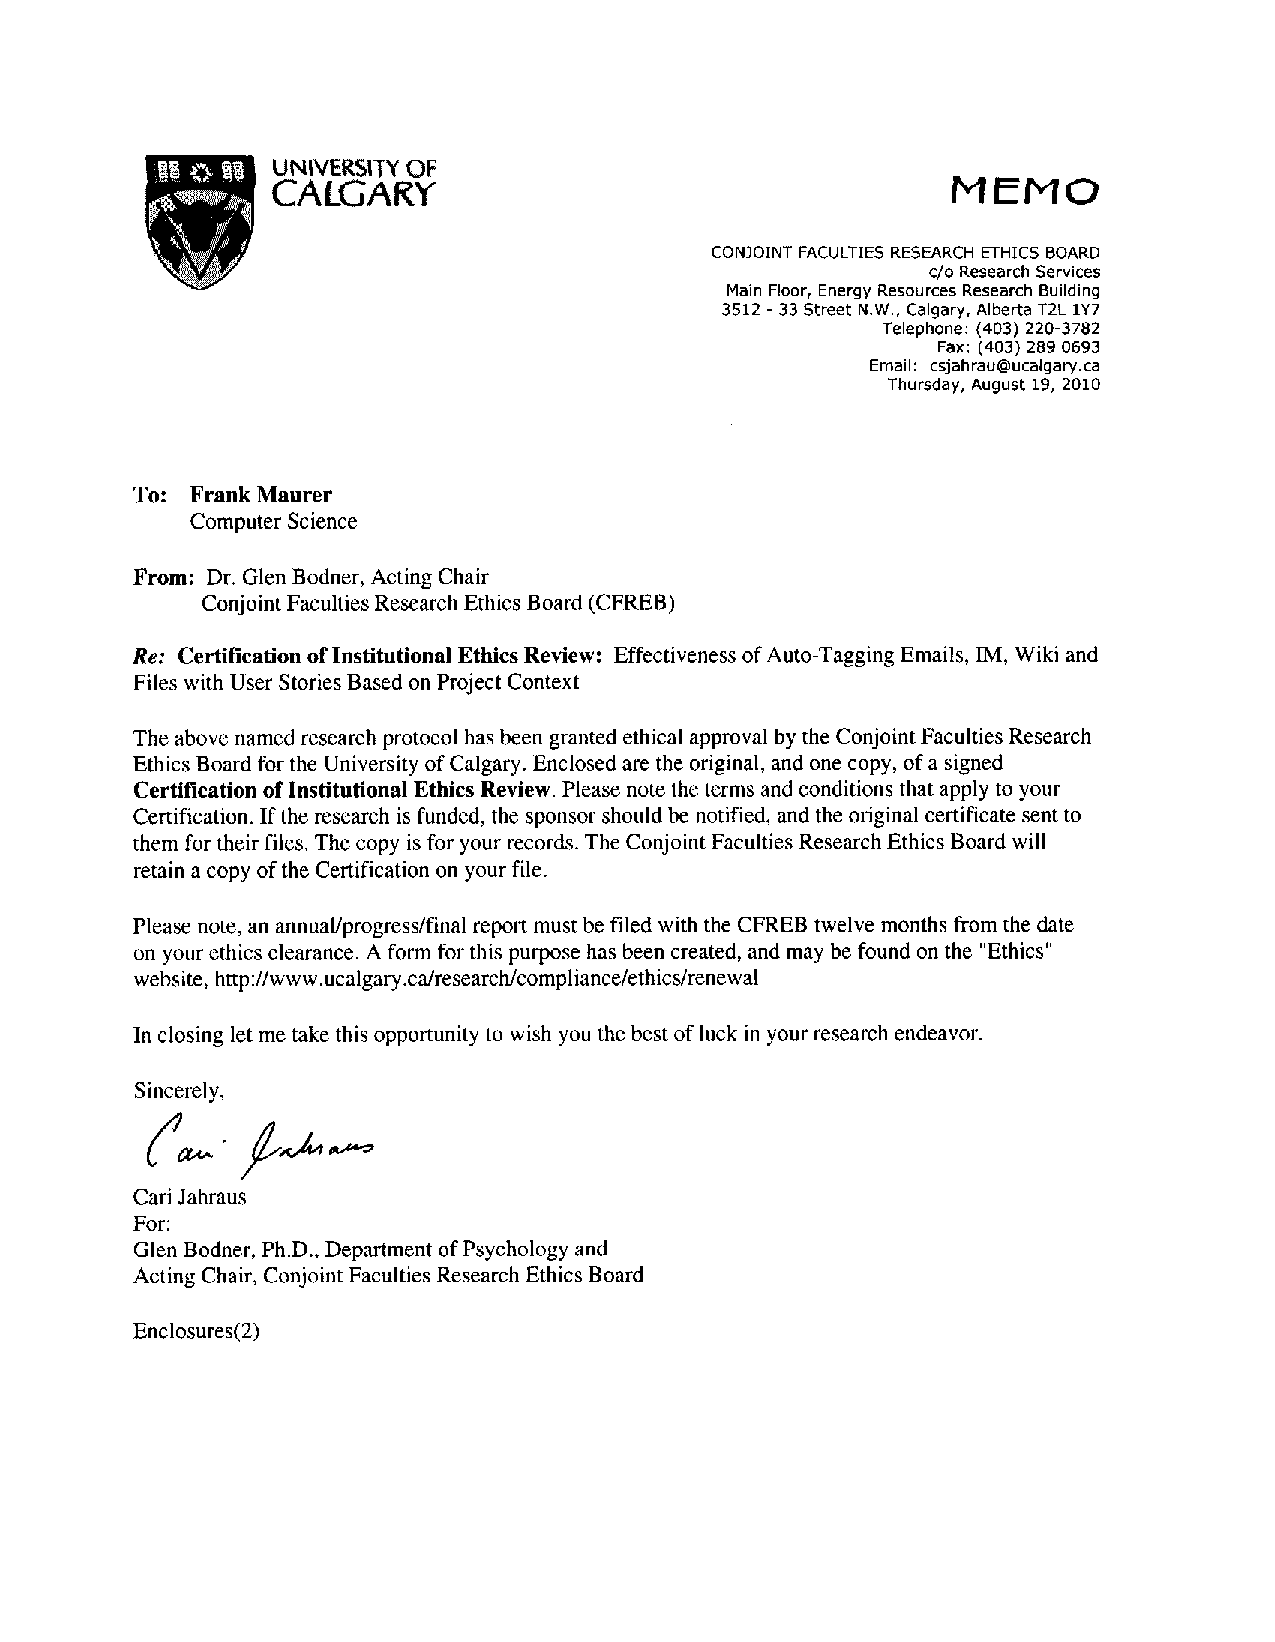
\includegraphics[width=\textwidth]{ethics.pdf}
    \caption{Ethics Approval}
	\label{fig:ethics}
\end{figure*}





\bibliographystyle{unsrt}
\bibliography{references}






\end{document}
